\documentclass{article}
\usepackage[utf8]{inputenc}
\usepackage[T2A,T1]{fontenc}
\usepackage[english,russian]{babel}
\usepackage{amsmath}
\usepackage{amssymb,amsfonts,textcomp}
\usepackage{fancyhdr}
\usepackage{array}
\usepackage{longtable}
\usepackage{hhline}
\usepackage[pdftex]{graphicx}
\usepackage[colorlinks=true,linkcolor=blue,unicode, pdftex]{hyperref}
\makeatletter
\newcommand\arraybslash{\let\\\@arraycr}
\makeatother
\setlength\tabcolsep{1mm}
\renewcommand\arraystretch{1.3}
\newcounter{Table}[section]
\renewcommand\theTable{\thesection.\arabic{Table}}
\parindent=1cm
\usepackage[letterpaper, left=3cm, right=2.5cm, top=2.5cm, bottom=2.5cm]{geometry}
\usepackage{color}
\usepackage{framed}
\usepackage{titlesec}
\usepackage{fancybox}
\usepackage[tikz]{bclogo}
\usepackage{xhfill}
\usepackage{booktabs}
\usepackage{listingsutf8}
\usepackage{float}
\usepackage{tablefootnote}
\usepackage{colortbl} 
\usepackage{type1ec} % для четкости шрифта
\usepackage[numbered]{bookmark} % для корректного отображения оглавления в ридере
\usepackage{arydshln} %для пунктирных линий
\usepackage[framemethod=tikz]{mdframed}
\usepackage{multirow}


\mdfsetup{%
	middlelinewidth=0.5pt,
	backgroundcolor=white!98!black,	
	roundcorner=5pt,
	innerleftmargin = 10pt,
	innertopmargin=5pt,
	skipabove = 10pt,
	skipbelow = 5pt,
	shadow=true,
	shadowsize=4pt,
	nobreak=false,
	rightmargin=0pt,
	align=right, 
}
\global\mdfdefinestyle{importantstyle}{%
	linecolor=red,linewidth=4pt,%
	topline=false,bottomline=false, rightline = false, %
	backgroundcolor=red!8,%
	shadow=false
}

\global\mdfdefinestyle{examplestyle}{%
	middlelinewidth=0.5pt,
	backgroundcolor=white!98!black,	
	roundcorner=5pt,
	innerleftmargin = 10pt,
	innertopmargin=5pt,
	skipabove = 10pt,
	skipbelow = 5pt,
	shadow=true,
	shadowsize=4pt,
	nobreak=false,
	rightmargin=0pt,
	align=right, 
}


\global\mdfdefinestyle{remarkstyle}{%
	linecolor=green!50!black,linewidth=4pt,%
	topline=false,bottomline=false, rightline = false, %
	backgroundcolor=green!8,%
	shadow=false
}

\mdfdefinestyle{theoremstyle}{%
	frametitlebackgroundcolor=white!40!black,
	frametitlealignment = \raggedright,
	frametitlerule=true,
	frametitlefont={\normalfont\bfseries\color{white}},
	frametitlebelowskip = 4pt,
	frametitleaboveskip = 4pt,
}


\newcounter{redlisting}[section]
\renewcommand{\theredlisting}{\thesection.\arabic{redlisting}}
\newcommand{\li}{\refstepcounter{redlisting} Листинг \theredlisting. }
\newcommand{\enli}{\refstepcounter{redlisting} Listing \theredlisting. }


\newenvironment{redlisting}[1]{\begin{mdframed}[style=theoremstyle,frametitle={\li #1}]\flushleft}{\end{mdframed}}

\newenvironment{redexample}{\begin{mdframed}\flushleft}{\end{mdframed}}

\newenvironment{redimportant}{\begin{mdframed}[style=importantstyle]}{\end{mdframed}}

\newenvironment{redremark}{\begin{mdframed}[style=remarkstyle]}{\end{mdframed}}


\usepackage{comment}

%\usepackage{parskip}
\usepackage{enumitem}

\usepackage{indentfirst}  % абзацный отступ после заголовка
\graphicspath{{SQLGuide-img/}} %

% другой счетчик для приложений (по \ref выдает A,B,C...)
\newcounter{application}
\renewcommand{\theapplication}{\Asbuk{application}}
\newcommand{\appcount}{\refstepcounter{application}}

\newcounter{test}
\renewcommand{\thetest}{\Asbuk{test}}
\newcommand{\apptest}{\refstepcounter{test}}

% чтобы в оглавлении было не присто А Б, а Приложение А, Приложение Б
\renewcommand\appendixname{Приложение}

\makeatletter
\def\redeflsection{\def\l@section{\@dottedtocline{1}{0em}{8em}}}
\renewcommand\appendix{\par
	\setcounter{application}{0}%
	\setcounter{subsection}{0}%
	\def\@chapapp{\appendixname}%
	\addtocontents{toc}{\protect\redeflsection}	
	\def\thesection{\appendixname\hspace{0.2cm}\Asbuk{application}}
	}
\makeatother


% чтобы разделы в оглавлении были не жирным а обычным шрифтом
\makeatletter 
\renewcommand*\l@section[2]{% 
	\ifnum \c@tocdepth >\z@ 
	\addpenalty\@secpenalty 
	\addvspace{1.0em \@plus\p@}% 
	\setlength\@tempdima{1.5em}% 
	\begingroup 
	\parindent \z@ \rightskip \@pnumwidth 
	\parfillskip -\@pnumwidth 
	\leavevmode 
	\advance\leftskip\@tempdima 
	\hskip -\leftskip 
	#1\nobreak\hfil \nobreak\hb@xt@\@pnumwidth{\hss #2}\par 
	\endgroup 
	\fi} 
\makeatother 


\emergencystretch=25pt %борьба с переполнением строк


\renewcommand{\thetable}{\thesection.\arabic{table}} % нумерация таблиц с номером section
\renewcommand{\thefigure}{\thesection.\arabic{figure}} % нумерация рисунков с номером section

\makeatletter
\@addtoreset{table}{section} % сбросит счетчик таблиц в начале каждого раздела. 
\makeatother

\makeatletter
\@addtoreset{figure}{section} % сбросит счетчик рисунков в начале каждого раздела. 
\makeatother

% пакет оформления блоков "Внимание" и "Пример"
\usepackage{tcolorbox}
\tcbuselibrary{most}

%пакет для работы с плавающими объектами
\usepackage{afterpage}

%оформление таблиц и рисунков по ГОСТ
\usepackage[tableposition=top]{caption}
\usepackage{subcaption}
\DeclareCaptionLabelFormat{gostfigure}{Рисунок #2} 
\DeclareCaptionLabelFormat{gosttable}{Таблица #2} 
\DeclareCaptionLabelSeparator{gost}{~---~}
\captionsetup{labelsep=gost}
\captionsetup[figure]{labelformat=gostfigure}
\captionsetup[table]{labelformat=gosttable,justification=raggedright,slc=off} 

\newcommand{\vspacebf}[1]{\vspace{5pt}\noindent \textbf{#1}}

%задает цвет гиперссылок 
\hypersetup{urlcolor=blue}

\tcbset{
	enhanced,
	colback=black!2,
	boxrule=0.4pt,
	fonttitle=\bfseries
}



%задает пустое пространство до и после таблицы
\setlength{\LTpre}{5pt}
\setlength{\LTpost}{5pt}

\newenvironment{redparam}
{\vspace{10pt}\bf\parindent=0cm}
{\par}

\newenvironment{redparam1}
{\vspace{5pt}\ttfamily\parindent=0cm}
{}


\newenvironment{rederror}
{\par\vspace{5pt}\ttfamily}
{\par\vspace{5pt}}

\newcommand{\sectionbreak}{\clearpage}

\titleformat{\section}
{\huge}
{\thesection}{1em}{}

\titleformat{\subsection}
{\LARGE}
{\thesubsection}{1em}{}

\titleformat{\subsubsection}
{\Large}
{\thesubsubsection}{1em}{}

\titleformat{\paragraph}
{\large}
{\theparagraph}{1em}{}

  
\title{}
\author{Red Soft Corporation}
\date{}

\setlength{\headheight}{24pt}
\pagestyle{fancy}


\newcommand{\anonsection}[1]{\phantomsection\section*{#1}\addcontentsline{toc}{section}{#1}}


\newcommand{\anonsubsection}[1]{\phantomsection\subsection*{#1}\addcontentsline{toc}{subsection}{#1}}

\newcommand{\anonsubsubsection}[2][]{\phantomsection%
	\subsubsection*{#2}%
	\ifthenelse{\equal{#1}{}}{\addcontentsline{toc}{subsubsection}{#2}}{\addcontentsline{toc}{subsubsection}{#1}}%
	}





\newcommand{\beginrudoc}[1]{
\fancyhf{}
\thispagestyle{empty}

\topskip0pt
\vspace*{\fill}

\begin{flushright}
\Huge {\xhrulefill{red}{2mm}\color{red} Red Expert} \\
\LARGE Версия 2020.10\\
#1
\end{flushright}

\vspace*{\fill}

\newpage

\fancyhead[R]{#1\\\rightmark}
\fancyfoot[C]{\xhrulefill{red}{2mm} Стр. \thepage}

\setcounter{tocdepth}{10}
\renewcommand\contentsname{Содержание}
\tableofcontents
}


%печать одинарных кавычек
\newcommand{\rr}[1]{{\textquotesingle}#1{\textquotesingle}}

%печать двойных кавычек
\newcommand{\pp}[1]{"#1{}"}

\newcommand{\ttt}{\texttt}

%для приложения 5 в SQL
\newcommand{\hl}[1]{\hyperlink{#1}{#1}}

\setlist[enumerate]{itemindent=1.3mm, topsep = 1mm, parsep=0pt, leftmargin=45pt} %чтобы списки были более сжатыми
\setlist[itemize]{itemindent=1.3mm, topsep = 1mm, parsep=0pt, leftmargin=45pt}   %чтобы списки были более сжатыми



\begin{document}

\beginrudoc{Руководство пользователя}

\anonsection{Введение}

Red Expert (Ред Эксперт) - это GUI-оболочка, предоставляющая интерфейс для работы с базами данных Firebird и Ред Базой Данных. Написанная полностью на Java, Red Expert является программой, независимой от операционной системы, для которой требуется только JDK не ниже 1.8.

Используя гибкость, предоставляемую Java Database Connectivity (JDBC), Red Expert обеспечивает простой способ взаимодействия с базой данных от простых запросов до создания таблиц и импорта / экспорта данных всей базе данных.

Red Expert был протестирован под Windows, Linux с использованием Java 1.8.

Red Expert обладает рядом полезных компонентов: визуальным редактором для всех объектов базы данных, редактором SQL запросов и исполнителем SQL скриптов и др.

\section{Обзор графического интерфейса}\label{sec:overview}

В Red Expert используется распространенный для таких инструментов и даже большинства IDE интерфейс с вкладками и подключаемыми компонентами.

На центральной панели окна приложения в виде вкладок размещаются основные функциональные компоненты, такие как:
\begin{itemize}
	\item \hyperref[sec:connections]{Браузер баз данных};
	\item \hyperref[sec:create_db]{Компонент для создания новой базы данных};
	\item \hyperref[sec:new_driver]{Компонент для установки JDBC драйверов};
	\item \hyperref[sec:objects]{Обозреватели и редакторы объектов базы данных};
	\item \hyperref[sec:query_editor]{Редактор запросов};
	\item \hyperref[sec:draft]{Черновик};
	\item \hyperref[sec:user_manager]{Менеджер пользователей};
	\item \hyperref[sec:priv_manager]{Менеджер прав}; 
	\item \hyperref[sec:trace_manager]{Трейс менеджер};
	\item \hyperref[sec:logout]{Обозреватель системного журнала состояний вывода};
	\item \hyperref[sec:erd]{Построитель ER-диаграмм};
	\item \hyperref[sec:compare_datatype]{Компонент для сравнения типов данных};
	\item \hyperref[sec:execute_proc]{Компонент для выполнения хранимых процедур и функций};
	\item \hyperref[sec:export_results]{Компонент для экспорта результатов SELECT запроса};
	\item \hyperref[sec:execute_scripts]{Компонент для выполнения скриптов из файла};
\end{itemize}

\begin{figure}[H]
	\centering
	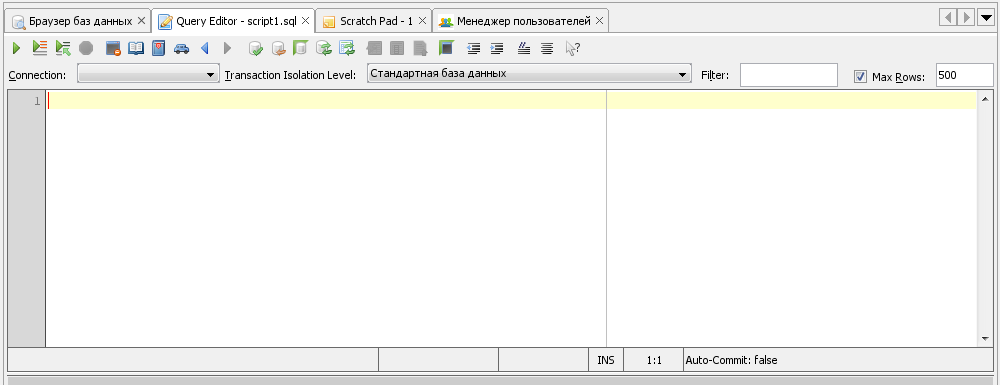
\includegraphics[width = 0.76\linewidth]{img/main_pane.png}
\end{figure}

Список всех открытых в настоящее время вкладок можно посмотреть, нажав на кнопку \begin{tikzpicture}
\pgftext{
\includegraphics[width=14pt]{img/button_alltabs.png}} at (0pt,0pt)
\end{tikzpicture} в правой части центральной панели.


Левая, нижняя и правая панели окна приложения предназначены для других подключаемых компонентов -- тех что описаны в разделе \hyperref[sec:dockable_panes]{Прикрепляемые панели}. Все эти компоненты можно перетащить в любую из трех позиций по желанию. Отображение компонентов настраивается через меню \textit{Вид}.

\hyperref[sec:toolbar]{Панель инструментов} в верхней части окна приложения также настраивается через меню \textit{Вид} и в \hyperref[sec:pref_toolbar]{настройках} приложения. Каждая группа инструментов может перемещаться горизонтально или вертикально вдоль области верхней панели.

\begin{figure}[H]
	\centering
	
\includegraphics[width = 0.75\linewidth]{img/toolbar.png}
\end{figure}

\section{Панель инструментов}\label{sec:toolbar}

Red Expert включает 6 основных групп панелей инструментов в верхней части окна приложения. Отдельные группы могут перемещаться горизонтально или вертикально вдоль верхней части окна приложения. Каждую группу инструментов можно скрыть или сделать видимой через меню \textit{Вид} или в \hyperref[sec:pref_toolbar]{настройках} приложения. 

Далее следует описание каждой панели инструментов и связанных с ней кнопок и действий. 

\begin{longtable}[c]{|m{5mm}|m{9cm}|>{\ttfamily}m{4cm}|}
	\caption{Панель инструментов для работы с файлами}\\
	\hline
	&
	\centering\bfseries Описание &
	\centering\arraybslash\normalfont\bfseries Горячие клавиши\\\hline
	\endfirsthead
	\hline
	&
	\centering\bfseries Описание &
	\centering\arraybslash\normalfont\bfseries Горячие клавиши\\\hline
	\endhead
	\begin{tikzpicture}
	\pgftext{\includegraphics[width=11pt]{img/new16.png}} at (0pt,0pt)
	\end{tikzpicture} & Новый документ & Shift+F12\\
	\hline
	\begin{tikzpicture}
	\pgftext{\includegraphics[width=14pt]{img/open16.png}} at (0pt,0pt)
	\end{tikzpicture} & Открыть файл & Ctrl+L\\
	\hline
	\begin{tikzpicture}
	\pgftext{\includegraphics[width=11pt]{img/save16.png}} at (0pt,0pt)
	\end{tikzpicture} & Сохранить файл & Ctrl+S\\
	\hline
	\begin{tikzpicture}
	\pgftext{\includegraphics[width=12pt]{img/print16.png}} at (0pt,0pt)
	\end{tikzpicture} & Печать & Ctrl+P\\
	\hline
	\begin{tikzpicture}
	\pgftext{
\includegraphics[width=12pt]{img/PrintPreview16.png}} at (0pt,0pt)
	\end{tikzpicture} & Предварительный просмотр перед печатью & \\
	\hline
	\begin{tikzpicture}
	\pgftext{
\includegraphics[width=11pt]{img/SaveAs16.png}} at (0pt,0pt)
	\end{tikzpicture} & Сохранить как & Ctrl+Shift+S\\
	\hline
	\begin{tikzpicture}
	\pgftext{
\includegraphics[width=12pt]{img/PageSetup16.png}} at (0pt,0pt)
	\end{tikzpicture} & Свойства печати &\\
	\hline
\end{longtable}

\begin{longtable}[c]{|m{5mm}|m{9cm}|>{\ttfamily}m{4cm}|}
	\caption{Панель инструментов для редактирования}\\
	\hline
	&
	\centering\bfseries Описание &
	\centering\arraybslash\normalfont\bfseries Горячие клавиши\\\hline
	\endfirsthead
	\hline
	&
	\centering\bfseries Описание &
	\centering\arraybslash\normalfont\bfseries Горячие клавиши\\\hline
	\endhead
	\begin{tikzpicture}
	\pgftext{\includegraphics[width=12pt]{img/cut16.png}} at (0pt,0pt)
	\end{tikzpicture} & Вырезать & Ctrl+X\\
	\hline
	\begin{tikzpicture}
	\pgftext{
\includegraphics[width=12pt]{img/Copy16.png}} at (0pt,0pt)
	\end{tikzpicture} & Копировать & Ctrl+C\\
	\hline
	\begin{tikzpicture}
	\pgftext{
\includegraphics[width=12pt]{img/Paste16.png}} at (0pt,0pt)
	\end{tikzpicture} & Вставить & Ctrl+V\\
	\hline
	\begin{tikzpicture}
	\pgftext{
\includegraphics[width=12pt]{img/Undo16.png}} at (0pt,0pt)
	\end{tikzpicture} & Отмена действий & Ctrl+Z\\
	\hline
	\begin{tikzpicture}
	\pgftext{
\includegraphics[width=12pt]{img/Redo16.png}} at (0pt,0pt)
	\end{tikzpicture} & Возврат отмененного действия & Ctrl+Y\\
	\hline
\end{longtable}	

\begin{longtable}[c]{|m{5mm}|m{9cm}|>{\ttfamily}m{4cm}|}
	\caption{Панель инструментов для работы с базой данных}\\
	\hline
	&
	\centering\bfseries Описание &
	\centering\arraybslash\normalfont\bfseries Горячие клавиши\\\hline
	\endfirsthead
	\hline
	&
	\centering\bfseries Описание &
	\centering\arraybslash\normalfont\bfseries Горячие клавиши\\\hline
	\endhead
	\begin{tikzpicture}
	\pgftext{
\includegraphics[width=12pt]{img/DBImage16.png}} at (0pt,0pt)
	\end{tikzpicture} & Создать подключение & Ctrl+Shift+N\\
	\hline
	\begin{tikzpicture}
	\pgftext{
\includegraphics[width=12pt]{img/Edit16.png}} at (0pt,0pt)
	\end{tikzpicture} & Редактор запросов & \\
	\hline
	\begin{tikzpicture}
	\pgftext{
\includegraphics[width=12pt]{img/create_database16.png}} at (0pt,0pt)
	\end{tikzpicture} & Создать базу данных & \\
	\hline
	\begin{tikzpicture}
	\pgftext{
\includegraphics[width=12pt]{img/NewTable16.png}} at (0pt,0pt)
	\end{tikzpicture} & Создать таблицу & \\
	\hline
	\begin{tikzpicture}
	\pgftext{
\includegraphics[width=12pt]{img/NewIndex16.png}} at (0pt,0pt)
	\end{tikzpicture} & Создать индекс & \\
	\hline
	\begin{tikzpicture}
	\pgftext{
\includegraphics[width=12pt]{img/CreateScripts16.png}} at (0pt,0pt)
	\end{tikzpicture} & Сгенерировать SQL скрипт & \\
	\hline
	\begin{tikzpicture}
	\pgftext{
\includegraphics[width=10pt]{img/Procedure16.png}} at (0pt,0pt)
	\end{tikzpicture} & Выполнить хранимые объекты & \\
	\hline
	\begin{tikzpicture}
	\pgftext{
\includegraphics[width=10pt]{img/user_manager_16.png}} at (0pt,0pt)
	\end{tikzpicture} & Менеджер пользователей & \\
	\hline
	\begin{tikzpicture}
	\pgftext{
\includegraphics[width=12pt]{img/grant_manager_16.png}} at (0pt,0pt)
	\end{tikzpicture} & Менеджер прав & \\
	\hline
	\begin{tikzpicture}
	\pgftext{
\includegraphics[width=12pt]{img/CompareDataTypes16.png}} at (0pt,0pt)
	\end{tikzpicture} & Сравнить типы данных & \\
	\hline
	\begin{tikzpicture}
	\pgftext{
\includegraphics[width=12pt]{img/Keywords16.png}} at (0pt,0pt)
	\end{tikzpicture} & Пользовательские ключевые слова & \\
	\hline
	\begin{tikzpicture}
	\pgftext{
\includegraphics[width=12pt]{img/SystemConsole16.png}} at (0pt,0pt)
	\end{tikzpicture} & Окно системной консоли & \\
	\hline
\end{longtable}	

\begin{longtable}[c]{|m{5mm}|m{9cm}|>{\ttfamily}m{4cm}|}
	\caption{Панель инструментов браузера}\\
	\hline
	&
	\centering\bfseries Описание &
	\centering\arraybslash\normalfont\bfseries Горячие клавиши\\\hline
	\endfirsthead
	\hline
	&
	\centering\bfseries Описание &
	\centering\arraybslash\normalfont\bfseries Горячие клавиши\\\hline
	\endhead
	\begin{tikzpicture}
	\pgftext{
\includegraphics[width=12pt]{img/ColumnInsertAfter16.png}} at (0pt,0pt)
	\end{tikzpicture} & Создать новый столбец в таблице после выделенного & \\
	\hline
	\begin{tikzpicture}
	\pgftext{
\includegraphics[width=12pt]{img/ColumnDelete16.png}} at (0pt,0pt)
	\end{tikzpicture} & Удалить выделенный столбец в таблице & Ctrl+C\\
	\hline
	\begin{tikzpicture}
	\pgftext{
\includegraphics[width=12pt]{img/DropTable16.png}} at (0pt,0pt)
	\end{tikzpicture} & Удалить выделенный объект & Ctrl+V\\
	\hline
\end{longtable}	

\begin{longtable}[c]{|m{5mm}|m{9cm}|>{\ttfamily}m{4cm}|}
	\caption{Панель инструментов для поиска}\\
	\hline
	&
	\centering\bfseries Описание &
	\centering\arraybslash\normalfont\bfseries Горячие клавиши\\\hline
	\endfirsthead
	\hline
	&
	\centering\bfseries Описание &
	\centering\arraybslash\normalfont\bfseries Горячие клавиши\\\hline
	\endhead
	\begin{tikzpicture}
	\pgftext{
\includegraphics[width=12pt]{img/Find16.png}} at (0pt,0pt)
	\end{tikzpicture} & Найти & Ctrl+F\\
	\hline
	\begin{tikzpicture}
	\pgftext{
\includegraphics[width=12pt]{img/FindAgain16.png}} at (0pt,0pt)
	\end{tikzpicture} & Найти далее & F3\\
	\hline
	\begin{tikzpicture}
	\pgftext{
\includegraphics[width=12pt]{img/Replace16.png}} at (0pt,0pt)
	\end{tikzpicture} & Заменить & Ctrl+R\\
	\hline
	\begin{tikzpicture}
	\pgftext{
\includegraphics[width=12pt]{img/GoTo16.png}} at (0pt,0pt)
	\end{tikzpicture} & Перейти к ... & Ctrl+G\\
	\hline
	\begin{tikzpicture}
	\pgftext{
\includegraphics[width=12pt]{img/FindInFiles16.png}} at (0pt,0pt)
	\end{tikzpicture} & Найти файлы & \\
	\hline
\end{longtable}	

\begin{longtable}[c]{|m{5mm}|m{9cm}|>{\ttfamily}m{4cm}|}
	\caption{Системные настройки}\\
	\hline
	&
	\centering\bfseries Описание &
	\centering\arraybslash\normalfont\bfseries Горячие клавиши\\\hline
	\endfirsthead
	\hline
	&
	\centering\bfseries Описание &
	\centering\arraybslash\normalfont\bfseries Горячие клавиши\\\hline
	\endhead
	\begin{tikzpicture}
	\pgftext{
\includegraphics[width=12pt]{img/Preferences16.png}} at (0pt,0pt)
	\end{tikzpicture} & Настройки & \\
	\hline
	\begin{tikzpicture}
	\pgftext{
\includegraphics[width=12pt]{img/Help16.png}} at (0pt,0pt)
	\end{tikzpicture} & Разделы справки & F1\\
	\hline
	\begin{tikzpicture}
	\pgftext{
\includegraphics[width=12pt]{img/About16.png}} at (0pt,0pt)
	\end{tikzpicture} & О программе & \\
	\hline
	\begin{tikzpicture}
	\pgftext{
\includegraphics[width=12pt]{img/WebComponent16.png}} at (0pt,0pt)
	\end{tikzpicture} & Посетить red-soft.ru & \\
	\hline
	\begin{tikzpicture}
	\pgftext{
\includegraphics[width=12pt]{img/ResourceHeap16.png}} at (0pt,0pt)
	\end{tikzpicture} & Состояние памяти & \\
	\hline
\end{longtable}


\section{Драйверы}\label{sec:drivers}

Red Expert использует информацию, доступную из установленных JDBC драйверов базы данных, для генерации большей части ее содержимого. 

По умолчанию в Red Expert уже установлена библиотека драйвера Jaybird 3 Driver, которая позволяет работать с базами данных Firebird и Ред Базой Данных.

\anonsubsection{Установка нового драйвера}\label{sec:new_driver}

\begin{redremark}
	Для получения информации о загрузке и использовании конкретных JDBC драйверов обратитесь к документации поставщиков баз данных.
\end{redremark}

\begin{enumerate}[leftmargin=15pt]
	\item Откройте панель \textit{Драйверы}, установив галочку в пункте меню \textit{Вид}.
	\item Откройте вкладку «Драйверы» на центральной панели (если вкладка не видна, кликните мышью по узлу «JDBC Drivers» панели  \textit{Драйверы}).
	\item Нажмите кнопку «New driver» на вкладке «Драйверы» или на кнопку 
	\begin{tikzpicture}
	\pgftext{
\includegraphics[width=14pt]{img/NewJDBCDriver16.png}} at (0pt,0pt)
	\end{tikzpicture}
	на панели инструментов компонента \textit{Драйверы}.
	\item Заполните соответствующие поля, как показано ниже:
	\begin{longtable}[r]{|>{\bfseries}m{3.5cm}|m{11.4cm}|}
		\hline
		Имя драйвера & Имя драйвера для идентификации\\\hline
		Описание & Краткое описание этого драйвера \\\hline
		База данных & Выберите СУБД, для которой этот драйвер предназначен\\\hline
		JDBC URL & Шаблон URL-адреса для этого JDBC драйвера. Например:
		\ttt{jdbc:firebirdsql://[host]:[port]/[source]} \\\hline
		Путь & Путь к jar-файлу JDBC-драйвера \\\hline
		Имя класса & Имя класса JDBC-драйвера. Выберите кнопку поиска, если имя неизвестно, и система сканирует файл jar, введенный в поле пути, для поиска имени класса драйвера\\\hline
	\end{longtable}
	\item Теперь драйвер готов к использованию и появится в списке доступных драйверов при подключении к базе данных в качестве имени, указанного выше.
\end{enumerate}

\section{Создание базы данных}\label{sec:create_db}
\begin{enumerate}[leftmargin=15pt]
	\item Откройте вкладку «Create Database» на центральной панели. Для этого выберите пункт меню \textit{База данных} $\rightarrow$ \textit{Создать базу данных}. Либо нажмите кнопку 
	\begin{tikzpicture}
	\pgftext{
\includegraphics[width=14pt]{img/create_database16.png}} at (0pt,0pt)
	\end{tikzpicture}
	на главной панели инструментов.
	\item Заполните соответствующие поля, как показано ниже:
	\begin{longtable}[r]{|>{\bfseries}m{3.9cm}|m{11cm}|}
		\hline
		JDBC драйвер & Выберите JDBC драйвер из выпадающего списка для создания новой базы данных. Для Ред Базы Данных и Firebird рекомендуется JDBC драйвер Jaybird 3 \\\hline
		Имя подключения & Имя подключения к этой базе данных \\\hline
		Имя сервера & Имя хоста сервера базы данных или IP-адрес\\\hline
		Порт & Номер порта подключения к базе данных \\\hline
		Файл базы данных & Путь к файлу базы данных или ее алиас\\\hline
		Имя пользователя & Логин пользователя, который в последствии станет владельцем базы данных\\\hline
		Пароль & Пароль пользователя \\\hline
		Сохранить пароль & Следует ли сохранять значение пароля с другой информацией о соединении\\\hline
		Зашифровать 
		
		пароль 	& Следует ли шифровать пароль при хранении, чтобы избежать открытого просмотра сохраненных паролей\\\hline
		Кодировка & Задает набор символов по умолчанию для строковых
		(символьных) данных для всей базы данных.  \\\hline
		Размер страницы & Размер страницы базы данных в байтах. Допустимыми значениями являются 4096, 8192 и 16384. \\\hline
	\end{longtable}
	
	\item Нажмите кнопку «Создать» для создания новой базы данных с введенные параметрами. 
\end{enumerate}	


\anonsubsection{Дополнительные параметры}

Дополнительные параметры соединения можно ввести, выбрав вкладку «Расширенные». На ней располагается таблица с двумя столбцами. Левый соответствует параметру подключения, а правый -- его значению. Обратитесь к соответствующей документации JDBC драйвера, чтобы узнать, какие (если есть) дополнительные параметры подключения к базе данных могут быть установлены.

Для драйвера Jaybird 3 в таблице \hyperref[tab:01]{ниже} перечислены основные параметры подключения.

Под таблицей предлагается выбрать уровень изоляции транзакций. Более подробно о них рассказано \hyperref[tab:isollevel]{далее}.

\section{Подключение к базе данных}\label{sec:connections}

Red Expert позволяет одновременно использовать несколько подключений к базе данных. Информация о подключении может быть получена через вкладку «Браузер базы данных». 

\anonsubsection{Создание нового подключения}

\begin{enumerate}[leftmargin=15pt]
	\item Убедитесь, что открыта панель \textit{Подключения} (если панель не открыта, установите галочку в пункте меню \textit{Вид} $\rightarrow$ \textit{Подключения}).
	\item Откройте вкладку «Браузер баз данных» на центральной панели (если вкладка не видна, кликните мышью по узлу «Подключения к базе данных» панели \textit{Подключения}).
	\item Нажмите кнопку «Новое подключение» на вкладке «Браузер баз данных» или кнопку 
	\begin{tikzpicture}
	\pgftext{
\includegraphics[width=14pt]{img/NewConnection16.png}} at (0pt,0pt)
	\end{tikzpicture}
	на панели инструментов компонента \textit{Подключения}.
	\item Заполните соответствующие поля, как показано ниже:
	\begin{longtable}[r]{|>{\bfseries}m{3.9cm}|m{11cm}|}
		\hline
		Состояние & Индикация, было ли установлено выбранное соединение - подключено или не подключено\\\hline
		JDBC драйвер & Выберите JDBC драйвер из выпадающего списка для этого подключения. Для Ред Базы Данных и Firebird рекомендуется JDBC драйвер Jaybird 3\\\hline
		Имя подключения & Имя подключения \\\hline
		Параметры
		
		подключения & Выпадающий список предлагает выбрать два способа подключения: 
		\begin{itemize}[leftmargin=10pt]
			\item Стандартно: отдельно указываются параметры подключения -- имя сервера, порт, файл БД, способ аутентификации, имя пользователя, пароль, кодировка и роль пользователя. 
			\item JDBC: по URL-адресу выбранного JDBC драйвера, например: \ttt{jdbc:firebirdsql://localhost:3050/employee?user=SYSDBA\& password=masterkey}
		\end{itemize}\\\hline
		Имя сервера & Имя хоста сервера базы данных или IP-адрес\\\hline
		Порт & Номер порта подключения к базе данных \\\hline
		Файл базы данных & Путь к файлу базы данных или ее алиас\\\hline
		Аутентификация & Способ аутентификации клиента:
		\begin{itemize}[leftmargin=10pt]
			\item Базовая: это традиционная (native для Ред Базы Данных 2.6; Legacy\_Auth для Ред Базы Данных 3.0) или безопасная парольная (Srp для Ред Базы Данных 3.0)
			\item Gss: доверенная (для Ред Базы Данных 3.0)
			\item Multifactor: многофакторная (для Ред Базы Данных)
		\end{itemize} 
		Если нужная аутентификация на сервере не включена или ее не существует, то будет выдано сообщение об ошибке о неверном логине-пароле. \\\hline
		Имя пользователя & Логин пользователя для подключения\\\hline
		Пароль & Пароль пользователя для подключения \\\hline
		Сохранить пароль & Следует ли сохранять значение пароля с другой информацией о соединении\\\hline
		Зашифровать 
		
		пароль 	& Следует ли шифровать пароль при хранении, чтобы избежать открытого просмотра сохраненных паролей\\\hline
		Кодировка & Набор символов для подключения \\\hline
		Роль & Роль подключающегося пользователя в текущей базе данных\\\hline
		JDBC URL & URL-адрес выбранного JDBC драйвера\\\hline
	\end{longtable}
	\item Нажмите кнопку «Подключиться», чтобы приложение попыталось установить соединение, используя введенные значения.
\end{enumerate}	

\anonsubsubsection{Расширенные параметры подключения}

Дополнительные свойства соединения можно ввести, выбрав вкладку «Расширенные». На ней можно увидеть таблицу с двумя столбцами. Левый соответствует параметру подключения, а правый -- его значению. Обратитесь к соответствующей документации JDBC драйвера, чтобы узнать, какие (если есть) дополнительные параметры подключения к базе данных могут быть установлены.

В таблице перечислены некоторый параметры для драйвера Jaybird 3: \label{tab:01}
\begin{longtable}[c]{|>{\ttfamily}m{4.2cm}|>{\ttfamily\centering}m{1.7cm}|m{9.5cm}|}
	\hline
	\centering\normalfont\bfseries Параметр &
	\centering\normalfont\bfseries Тип значения&
	\centering\arraybslash\bfseries Описание\\\hline
	\endfirsthead
	\hline
	\centering\normalfont\bfseries Параметр &
	\centering\normalfont\bfseries Тип значения &
	\centering\arraybslash\bfseries Описание\\\hline
	\endhead
	isc\_dpb\_user\_name & string & Имя подключающегося пользователя\\\hline
	isc\_dpb\_password & string & Пароль пользователя\\\hline
	isc\_dpb\_sql\_role\_name & string & Имя роли\\\hline
	isc\_dpb\_sql\_dialect & byte & SQL диалект \\\hline
	isc\_dpb\_process\_id & int & ID процесса \\\hline
	isc\_dpb\_process\_name & string & Имя процесса \\\hline
	isc\_dpb\_lc\_ctype & string & Кодировка символов соединения. Этот параметр сообщает серверу базы данных в какой кодировке клиент ждет строки и текст.\\\hline
	isc\_dpb\_connect\_timeout & int & Время ожидания подключения (в секундах)\\\hline
	isc\_dpb\_gss & -- & Использовать доверительную аутентификацию Gss\\\hline
	isc\_dpb\_num\_buffers & int & Количество страниц базы данных, которые будут кэшироваться\\\hline
	isc\_dpb\_set\_db\_readonly & boolean & Установить базу данных в режим только для чтения\\\hline
	isc\_dpb\_set\_db\_charset & string & Установить набор символов для базы данных \\\hline
	isc\_dpb\_trusted\_auth & -- & Информирование, что будет использоваться доверительная аутентификация\\\hline
	isc\_dpb\_multi\_factor\_ auth & boolean &  Информирование, что будет использоваться многофакторная аутентификация\\\hline
	isc\_dpb\_utf8\_filename  & -- & Информирование, что имя файла передается в формате UTF-8\\\hline
	isc\_dpb\_certificate & string & Алиас сертификата клиента при многофакторном подключении\\\hline
	isc\_dpb\_verify\_server & -- & Флаг для проверки сертификата сервера (многофакторная аутентификация) \\\hline
	isc\_dpb\_repository\_pin & string & Пин код для контейнера с сертификатом (многофакторная аутентификация)\\\hline
\end{longtable} 

Ниже под таблицей предлагается выбрать уровень изоляции транзакций. Различные уровни изоляции транзакций определяют поведение данного клиентского приложения, запустившего эту транзакцию, по отношению к другим параллельным процессам, выполняющимся на любом компьютере локальной сети, одновременно выполняющих чтение и/или изменение в той же базе данных, что и текущий процесс. 

Для транзакций существует несколько типов чтения:
\begin{itemize}
	\item \textit{Грязное чтение} (\ttt{dirty reads}) происходит, когда транзакциям разрешено видеть несохраненные изменения данных. Иными словами, изменения, сделанные в одной транзакции, видны вне ее до того, как она была сохранена. Если изменения не будут сохранены, то, вероятно, другие транзакции выполняли работу на основе некорректных данных;
	\item \textit{Неповторяющееся чтение} (\ttt{non-repeatable reads}) происходит, когда транзакция А читает строку, транзакция Б изменяет эту строку, транзакция А читает ту же строку и получает обновленные данные;
	\item \textit{Фантомное чтение} (\ttt{phantom reads}) происходит, когда транзакция А считывает все строки, удовлетворяющие \ttt{WHERE}-условию, транзакция Б вставляет новую или удаляет одну из строк, которая удовлетворяет этому условию, транзакция А еще раз считывает все строки, удовлетворяющие \ttt{WHERE}-условию, уже вместе с новой строкой или недосчитавшись старой.
\end{itemize}

Уровни изоляции транзакций определены в виде констант по возрастанию уровня ограничения: 
\begin{longtable}[c]{|>{\ttfamily}m{5.2cm}|m{10.2cm}|}
	\hline
	\centering\normalfont\bfseries Уровень изоляции &
	\centering\arraybslash\bfseries Описание\\\hline
	\endfirsthead
	\hline
	\centering\normalfont\bfseries Уровень изоляции &
	\centering\arraybslash\bfseries Описание\\\hline
	\endhead
	Стандартная база данных & Уровень изоляции по умолчанию, который установлен для данной базы данных. Для Ред Базы Данных и Firebird это \ttt{READ\_COMMITED}\\\hline
	TRANSACTION\_NONE & Информирует о том, что драйвер не поддерживает транзакции\\\hline
	TRANSACTION\_READ\_UNCOMMITED & Позволяет транзакциям видеть несохраненные изменения данных, что разрешает грязное, неповторяющееся и фантомное чтения\\\hline
	TRANSACTION\_READ\_COMMITED & Означает, что любое изменение, сделанное в транзакции, не видно вне неё, пока она не сохранена. Это предотвращает грязное чтение, но разрешает неповторяющееся и фантомное\\\hline
	TRANSACTION\_REPEATABLE\_READ & Запрещает грязное и неповторяющееся, но фантомное чтение разрешено\\\hline
	TRANSACTION\_SERIALIZABLE & Определяет, что грязное, неповторяющееся и фантомное чтения запрещены\\\hline
\end{longtable} 	


\anonsubsubsection{SSH туннель}\label{tab:isollevel}

Есть удобная возможность подключиться к базе данных через SSH-туннель. Как и при любом SSH-соединении, весь трафик между вами и БД будет шифроваться.

Для этого введите параметры подключения на вкладке «Базовые», переключитесь на вкладку «SSH Тоннель» и заполните параметры для SSH-соединения. Имя хоста переносится с вкладки «Базовые».


\anonsubsection{Закрытие соединения}

Подключение можно разорвать в любой момент, нажав на кнопку «Отключиться» на вкладке «Браузер баз данных». Есть и другой способ. На боковой панели \textit{Подключения} щелкните правой кнопкой мыши на нужное соединение и выберите пункт всплывающего меню \textit{Отключиться от базы данных <имя подключения>}.

\anonsubsection{Свойства базы данных}

После подключения к базе данных становится активной вкладка «Свойства базы данных». На ней располагается таблица с информацией о возможностях конкретной СУБД в сочетании с конкретным JDBC драйвером. Описание отдельных свойств см.~\hyperref[app:1]{Приложение~\ref{app:1}}

\anonsubsection{Ключевые слова SQL}

После подключения к базе данных становится активной вкладка «Ключевые слова SQL». На ней в одной из таблиц перечислены ключевые слова, определенные в стандарте SQL92, в другой -- определённые для конкретной СУБД.

Ключевые слова нельзя использовать в качестве имен объектов базы данных, переменных и параметров. 

\section{Редактор запросов}\label{sec:query_editor}

Чтобы открыть редактор запросов в центральной панели, выберите пункт меню \textit{Инструменты} $\rightarrow$ \textit{Редактор запросов} или нажмите кнопку \begin{tikzpicture}
\pgftext{
\includegraphics[width=12pt]{img/Edit16.png}} at (0pt,0pt)
\end{tikzpicture} 
на главной панели инструментов. Он открывается в виде вкладки с названием \textit{Query Editor -- script<N>.sql}. Файл с запросами к базе данных \ttt{script<N>.sql} можно сохранить (по умолчанию файл сохраняется в \ttt{\$HOME\textbackslash .redexpert\textbackslash2000\textbackslash QueryEditor}). 

Редактор запросов представляет собой настраиваемый инструмент просмотра и выполнения операторов SQL. В любой момент времени может быть открыто любое количество редакторов.

Редактор поддерживает следующие функции:
\begin{itemize}
	\item Настраиваемая подсветка синтаксиса SQL;
	\item Согласованность скобок;
	\item Подсказки ключевых слов и имен объектов базы данных по нажатию \ttt{Ctrl+Space};
	\item Выполнение нескольких запросов;
	\item Выполнение и отображение нескольких запросов с множеством результатов (\hyperref[sec:resultset]{Result Set});
	\item Поддержка \hyperref[sec:param_queries]{параметризованных запросов};
	\item Полная поддержка печати;
	\item Управление транзакциями;
	\item Функции текстового редактора стиля IDE - поиск, замена, вставка и т.д.;
	\item Экспорт результатов;
	\item Поддержка нескольких открытых соединений;
	\item Поисковая исполняемая \hyperref[sec:query_history]{история} SQL-запросов;
	\item Быстрый переход из редактора к просмотру объекта базы данных двойным кликом или нажатием \ttt{CTRL + Левая клавиша мыши} по имени объекта.
\end{itemize}

\anonsubsection{Панель инструментов}

Следующие команды доступны на панели инструментов редактора запросов:

\begin{longtable}[c]{|m{5mm}|m{10.6cm}|>{\ttfamily}m{4cm}|}
	\hline
	&
	\centering\bfseries Описание &
	\centering\arraybslash\normalfont\bfseries Горячие клавиши\\\hline
	\endfirsthead
	\hline
	&
	\centering\bfseries Описание &
	\centering\arraybslash\normalfont\bfseries Горячие клавиши\\\hline
	\endhead
	\begin{tikzpicture}
	\pgftext{
\includegraphics[width=12pt]{img/Execute16.png}} at (0pt,0pt)
	\end{tikzpicture} & Выполнить все операторы в редакторе & Ctrl+Shift+Enter\\\hline
	\begin{tikzpicture}
	\pgftext{
\includegraphics[width=12pt]{img/PartialExecute16.png}} at (0pt,0pt)
	\end{tikzpicture} & Выполнить оператор, на котором находится курсор (операторы должны быть разделены хотя бы одной пустой строкой) & Ctrl+Enter\\\hline
	\begin{tikzpicture}
	\pgftext{
\includegraphics[width=12pt]{img/ExecuteSelection16.png}} at (0pt,0pt)
	\end{tikzpicture} & Выполнить любой выделенный текст в редакторе & F9\\\hline
	\begin{tikzpicture}
	\pgftext{
\includegraphics[width=12pt]{img/plan.png}} at (0pt,0pt)
	\end{tikzpicture} & Печать плана запроса & Ctrl+Shift+P\\\hline
	\begin{tikzpicture}
	\pgftext{
\includegraphics[width=12pt]{img/Stop16.png}} at (0pt,0pt)
	\end{tikzpicture} & Отмена выполнения текущего оператора & \\\hline
	\begin{tikzpicture}
	\pgftext{
\includegraphics[width=12pt]{img/ClearOutput16.png}} at (0pt,0pt)
	\end{tikzpicture} & Очистить окно вывода (окно Output) & Ctrl+Shift+Backspace\\\hline
	\begin{tikzpicture}
	\pgftext{\includegraphics[width=12pt]{img/History16.png}} at (0pt,0pt)
	\end{tikzpicture} & Показать диалоговое окно истории выполненных запросов & Ctrl+Shift+H\\\hline
	\begin{tikzpicture}
	\pgftext{\includegraphics[width=12pt]{img/Bookmarks16.png}} at (0pt,0pt)
	\end{tikzpicture} & Закладки для хранения запросов. Для удобного поиска важных запросов  & Ctrl+B\\\hline
	\begin{tikzpicture}
	\pgftext{\includegraphics[width=12pt]{img/Shortcut16.png}} at (0pt,0pt)
	\end{tikzpicture} & Сокращения запросов. Появляется диалоговое окно, в котором можно найти или создать новое сокращение для определенных запросов к базе данных & \\\hline
	\begin{tikzpicture}
	\pgftext{\includegraphics[width=12pt]{img/Previous16.png}} at (0pt,0pt)
	\end{tikzpicture} & Показать в редакторе предыдущий выполненный запрос  & Ctrl+Shift+Down\\\hline
	\begin{tikzpicture}
	\pgftext{\includegraphics[width=12pt]{img/Forward16.png}} at (0pt,0pt)
	\end{tikzpicture} & Показать в редакторе следующий выполненный запрос  & Ctrl+Shift+Up\\\hline
	\begin{tikzpicture}
	\pgftext{\includegraphics[width=12pt]{img/Commit16.png}} at (0pt,0pt)
	\end{tikzpicture} & Коммит всех изменений с последнего коммита/отката  & Ctrl+Shift+C\\\hline
	\begin{tikzpicture}
	\pgftext{\includegraphics[width=12pt]{img/Rollback16.png}} at (0pt,0pt)
	\end{tikzpicture} & Отменить все изменения с последнего коммита/отката  & Ctrl+Shift+R\\\hline
	\begin{tikzpicture}
	\pgftext{\includegraphics[width=12pt]{img/AutoCommit16.png}} at (0pt,0pt)
	\end{tikzpicture} & Переключатель режима ручной/авто -- коммит. Если режим автокоммита выключен, то для подтверждения или отката транзакций следует нажимать кнопки \begin{tikzpicture}
	\pgftext{\includegraphics[width=12pt]{img/Commit16.png}} at (0pt,0pt)
	\end{tikzpicture} или  \begin{tikzpicture}
	\pgftext{\includegraphics[width=12pt]{img/Rollback16.png}} at (0pt,0pt)
	\end{tikzpicture} соответственно или прописывать команды \ttt{commit} или \ttt{rollback}. Если же режим автокоммита включен, то каждый оператор будет закоммичен по мере его выполнения. & \\\hline
	\begin{tikzpicture}
	\pgftext{\includegraphics[width=12pt]{img/RecycleConnection16.png}} at (0pt,0pt)
	\end{tikzpicture} & Закрытие соединения, выделенного для редактора запросов, и его повторное открытие & \\\hline
	\begin{tikzpicture}
	\pgftext{\includegraphics[width=12pt]{img/TableRefresh16.png}} at (0pt,0pt)
	\end{tikzpicture} & Обновить список ключевых слов & Alt+Shift+R\\\hline
	\begin{tikzpicture}
	\pgftext{\includegraphics[width=12pt]{img/RSMetaData16.png}} at (0pt,0pt)
	\end{tikzpicture} & Отображает метаданные выбранного множества результатов (Result Set) & \\\hline
	\begin{tikzpicture}
	\pgftext{\includegraphics[width=12pt]{img/TableColumn16.png}} at (0pt,0pt)
	\end{tikzpicture} & Показывает диалоговое окно, в котором можно выбрать какие столбцы выборки скрыть & \\\hline
	\begin{tikzpicture}
	\pgftext{\includegraphics[width=12pt]{img/ExportDelimited16.png}} at (0pt,0pt)
	\end{tikzpicture} & Экспорт выборки в файл & \\\hline
	\begin{tikzpicture}
	\pgftext{\includegraphics[width=12pt]{img/ToggleEditorOutput16.png}} at (0pt,0pt)
	\end{tikzpicture} & Показать/скрыть окно вывода & \\\hline
	\begin{tikzpicture}
	\pgftext{\includegraphics[width=12pt]{img/ShiftTextLeft16.png}} at (0pt,0pt)
	\end{tikzpicture} & Сдвиг текущей строки влево & \\\hline
	\begin{tikzpicture}
	\pgftext{\includegraphics[width=12pt]{img/ShiftTextRight16.png}} at (0pt,0pt)
	\end{tikzpicture} & Сдвиг текущей строки вправо & \\\hline
	\begin{tikzpicture}
	\pgftext{\includegraphics[width=12pt]{img/AddComment16.png}} at (0pt,0pt)
	\end{tikzpicture} & Закомментировать текущую строку или выделение & Ctrl+/\\\hline
	\begin{tikzpicture}
	\pgftext{\includegraphics[width=12pt]{img/FormatSql16.png}} at (0pt,0pt)
	\end{tikzpicture} & Форматирование SQL кода & Ctrl+Shift+F\\\hline
	\begin{tikzpicture}
	\pgftext{\includegraphics[width=12pt]{img/ContextualHelp16.png}} at (0pt,0pt)
	\end{tikzpicture} & Вызов справки по Редактору запросов & \\\hline
\end{longtable}	

\begin{longtable}[c]{|>{\ttfamily}m{2.8cm}|m{12.5cm}|}
	\hline
	Connection & Подключение к базе данных может быть изменено, используя выпадающий список всех доступных соединений \\\hline
	Transaction Isolation Level & Уровень изоляции транзакций можно поменять в текущем окне редактора запросов \\\hline
	Filter & Фильтрация записей в Result Set. Выполните запрос, который вернет множество результатов. Введите в фильтр искомое значение и нажмите \ttt{Enter} --- в новой вкладке откроются совпадающие с фильтром записи. \\\hline
	Max Rows & Урезает выборку до заданного количества строк \\\hline
\end{longtable}	

\anonsubsection{Панель Вывода}

Панель вывода редактора запросов представляет собой интерфейс с вкладками, отображающими сообщения о выполнении SQL запросов (информация, предупреждения, ошибки и т.д.) и результирующие наборы (Result Set).

При выполнении любого запроса в окне \textit{Output} будет логгироваться информация: о текущем подключении, содержимое SQL запроса, сообщения об успешном выполнении и ошибках, планы запросов и время выполнения.

Панель может быть очищена от ее содержимого в любое время, используя кнопку \begin{tikzpicture}
\pgftext{\includegraphics[width=12pt]{img/ClearOutput16.png}} at (0pt,0pt)
\end{tikzpicture} на панели инструментов редактора или через всплывающее меню по нажатию правой кнопки мыши.

Содержимое окна вывода редактора может сохраняться в файл. Для это откройте настройки редактора (\textit{Инструменты}$\rightarrow$\textit{Настройки}$\rightarrow$\textit{Editor}) и поставьте галочку напротив параметра «\ttt{Log output to file}». А в качестве значения параметра  «\ttt{Output log file path}» укажите путь к лог-файлу, в который будет записываться вывод.

\anonsubsubsection{Result Set}\label{sec:resultset}

Если результатом запроса является Result Set, то он отображается в отдельной вкладке на панели вывода. Если таких запросов несколько, то для каждого создается своя вкладка в порядке выполнения.

При наведении курсором мыши на открытую вкладку \textit{Result Set <N>} вылезает всплывающее окно с запросом, который выдал данный результат. Можно перейти к строке с этим запросом в редакторе, нажав на кнопку 
\begin{tikzpicture}
\pgftext{\includegraphics[width=12pt]{img/GoToResultSetQuery16.png}} at (0pt,0pt)
\end{tikzpicture} или скопировать его в буфер обмена. 

Над самой таблицей с выборкой также можно производить некоторые действия:
\begin{itemize}
	\item сортировать по полю, щелкнув мышью по заголовку нужного столбца
	\item перемещать в разном порядке столбцы таблицы
	\item скопировать выделенные строки или столбцы (см. всплывающее меню)
	\item экспортировать выделенное/таблицу в файл (см. всплывающее меню)
	\item скрыть некоторые поля выборки (см. всплывающее меню)
	\item печать выделенного или всей таблицы (см. всплывающее меню)
	\item посмотреть метаданные результирующей таблицы, нажав на кнопку \begin{tikzpicture}
	\pgftext{\includegraphics[width=12pt]{img/RSMetaData16.png}} at (0pt,0pt)
	\end{tikzpicture} на панели инструментов.
	
	\begin{redremark}
		Эта функция недоступна по умолчанию и должна быть включена в настройках приложения.
	\end{redremark}
\end{itemize}

\anonsubsection{Параметризованные запросы}\label{sec:param_queries}

В некоторых случаях нужно создать запрос, который можно использовать многократно, но каждый раз с разными «входными» значениями. Например, можно написать несколько запросов, чтобы найти данные о сотруднике с определенной фамилией. А можно написать один запрос, меняя только фамилию сотрудника.

Чтобы создать запрос, который в разное время может иметь разные «входные» данные, используются параметры запроса. Параметры могут быть именованными или неименованными. Неименованный параметр — это вопросительный знак («?»), который можно подставлять в любое место запроса, вместо литерального значения. Например:

\begin{redexample}\ttfamily
SELECT * FROM employees WHERE (surname = ?)  
\end{redexample}

Запустив на выполнение такой запрос в редакторе запросов, на экране появится диалоговое окно для ввода значения параметра (фамилии сотрудника):

\begin{figure}[H]
	\centering
	\includegraphics[width = 0.4\linewidth]{img/input_param.png}
\end{figure}

Именованные параметры -- это комбинация двоеточия и имени параметра (\ttt{:<paramname>}), которую также можно подставлять вместо литерального значения. Именованные параметры особенно полезны, если в запросе имеется несколько параметров. Например:

\begin{redexample}\ttfamily
	SELECT * FROM employees WHERE (surname = :surname AND name =:name)  
\end{redexample}

Запустив на выполнение такой запрос в редакторе запросов, на экране появится диалоговое окно для ввода значений параметров (фамилии и имени сотрудника):

\begin{figure}[H]
	\centering
	\includegraphics[width = 0.4\linewidth]{img/input_param2.png}
\end{figure}

\anonsubsection{История запросов}\label{sec:query_history}

После успешного выполнения любого запроса, он сохраняется в кеше журнала редактора для последующего удобного поиска поиска. Количество хранящихся в истории запросов указывается в настройках редактора. Сохраненные запросы не теряются после перезапуска приложения или редактора запросов

Чтобы посмотреть все сохраненные запросы, нажмите на кнопку 
\begin{tikzpicture}
\pgftext{\includegraphics[width=12pt]{img/History16.png}} at (0pt,0pt)
\end{tikzpicture} 
на панели инструментов редактора. Появится диалоговое окно, в котором можно воспользоваться строкой поиска нужного запроса, вставить его в открытое или новое окно редактора (весь текст открытого редактора будет перезаписан выбранным текстом запроса), вставить сохраненный запрос в место позиции курсора, копировать в буфер обмена текст запроса, очистить всю историю. 

Кэш истории можно прокручивать с помощью кнопок 
\begin{tikzpicture}
\pgftext{\includegraphics[width=12pt]{img/Previous16.png}} at (0pt,0pt)
\end{tikzpicture} 
и 
\begin{tikzpicture}
\pgftext{\includegraphics[width=12pt]{img/Forward16.png}} at (0pt,0pt)
\end{tikzpicture} на панели инструментов редактора. 


\section{Объекты}\label{sec:objects}

\anonsubsection{ИНДЕКСЫ}
\anonsubsubsection{Создание индексов}\label{sec:crind}

Диалоговое окно \textit{Create Index} позволяет создавать новые индексы таблиц базы данных в выбранном соединении с базой данных.

\begin{enumerate}[leftmargin=26pt]
	\item Выберите пункт меню \textit{База данных}$\rightarrow$\textit{Создать индекс} или кнопку 
	\begin{tikzpicture}
	\pgftext{\includegraphics[width=12pt]{img/NewIndex16.png}} at (0pt,0pt)
	\end{tikzpicture}
	на главной панели инструментов. Откроется диалоговое окно.
	\begin{figure}[H]
		\centering
		\includegraphics[width = 0.75\linewidth]{img/create_index.png}
	\end{figure}	
	\item Выберите открытое соединение с базой данных.
	\item Введите уникальное имя индекса.
	\item Выберите таблицу базы данных, для которой создается индекс.
	\item Выберите направление индекса (по возрастанию или по убыванию значений ключей индекса).
	\item Для уникальности значений индекса поставьте галочку на параметре \textit{Уникальный}.
	\item Чтобы перевести индекс в активное состояние, поставьте галочку на параметре \textit{Активный}. Иначе индекс будет переведен в неактивное состояние.
	\item Выберите столбцы выбранной таблицы для построения индекса или, если вы хотите построить вычисляемый индекс, поставьте галочку на поле \textit{Вычисляемое как} и впишите выражение.
	\item Напишите комментарий к индексу, если это необходимо.
	\item Нажмите кнопку \textit{OK}. Появится новое диалоговое окно для подтверждения или отката операции создания индекса (см. \hyperref[ris:01]{рис.~\ref{ris:01}}).
	\item Проверьте сгенерированный SQL код.
	\item Сделайте \ttt{commit} или \ttt{rollback} транзакции, нажав на соответствующие кнопки.
\end{enumerate}

\begin{figure}[H]
	\caption{Диалоговое окно подтверждения или отката DDL операций}\label{ris:01}
	\centering
	\includegraphics[width = 0.48\linewidth]{img/create_index2.png}
\end{figure}

\anonsubsubsection{Изменение индексов}
На боковой панели \textit{Подключения} щелкните правой кнопкой мыши по имени индекса и выберите пункт всплывающего меню \textit{Редактировать <имя индекса>:INDEX}. Откроется диалоговое окно \textit{Alter Index}. Алгоритм редактирования индекса полностью аналогичен его \hyperref[sec:crind]{созданию}.

\anonsubsubsection{Удаление индексов}
На боковой панели \textit{Подключения} щелкните правой кнопкой мыши по имени индекса и выберите пункт всплывающего меню \textit{Удалить <имя индекса>:INDEX}. Откроется  диалоговое окно для подтверждения или отката операции удаления индекса (см. \hyperref[ris:01]{рис.~\ref{ris:01}}). Для подтверждения операции нажмите кнопку «Подтвердить».

\anonsubsection{ПРОЦЕДУРЫ}

\anonsubsubsection{Создание процедур}\label{sec:crproc}
Диалоговое окно \textit{Create Procedure} позволяет создавать новые процедуры в выбранном соединении с базой данных.
\begin{enumerate}[leftmargin=26pt]
	\item На боковой панели \textit{Подключения} щелкните правой кнопкой мыши по объекту \textit{ПРОЦЕДУРЫ} и выберите пункт \textit{Создать PROCEDURE} всплывающего меню. Откроется диалоговое окно.
	\begin{figure}[H]
		\centering
		\includegraphics[width = 0.7\linewidth]{img/create_proc.png}
	\end{figure}
	\item Выберите открытое соединение с базой данных.
	\item Введите уникальное имя процедуры.
	\item На вкладке \textit{Edit} можно заполнить таблицы с входными, выходными параметрами и локальными переменными процедуры. \begin{longtable}[r]{|>{\ttfamily}m{3cm}|m{11.5cm}|}
		\hline
		\centering\normalfont\bfseries Имя столбца &
		\centering\arraybslash\bfseries Описание\\\hline
		\endfirsthead
		\hline
		\centering\normalfont\bfseries Имя столбца &
		\centering\arraybslash\bfseries Описание\\\hline
		\endhead
		Name & Имя параметра, может содержать до 31 байта \\\hline
		Datatype & Тип данных SQL параметра\\\hline
		Type of & Используется только с доменом. Если стоит галочка, значит используется только тип данных домена — не проверяется его ограничение (если оно есть в домене) на \ttt{NOT NULL, CHECK} ограничения и/или значения по умолчанию. \\\hline
		Domain & Имя домена в качестве типа параметра\\\hline
		Table & Имя таблицы, если в качестве типа параметра используется тип данных столбцов существующих таблиц.\\\hline
		Column & Имя столбца, если в качестве типа параметра используется тип данных столбцов существующих таблиц.\\\hline
		Size	 & Максимальный размер строки в символах (для строковых типов) Или точность от 1 до 18 для типов данных \ttt{DECIMAL, NUMERIC}. Или размер сегмента (не может превышать 65535) для типа данных \ttt{BLOB}.\\\hline
		Scale	 & Масштаб  для типов данных \ttt{DECIMAL, NUMERIC}. От 0 до 18, должно быть меньше или равно \ttt{Size} \\\hline
		Subtype	 &  Номер подтипа \ttt{BLOB}. \\\hline
		Description	 &  Добавление комментария для параметра процедуры\\\hline
		Default Value	 & Значение по умолчанию для параметра процедуры \\\hline
		Encoding & Кодировка для строковых типов \\\hline	
		Required & Запретить передавать в параметр значение \ttt{NULL}.\\\hline	
	\end{longtable}	
	\item На вкладке \textit{Edit} в поле ввода напишите тело процедуры.
	\item На вкладке \textit{Description} напишите комментарий к процедуре, если это необходимо.
	\item На вкладке \textit{DDL} проверьте сгенерированный SQL код и в случае необходимости исправьте его. 
	\item Нажмите кнопку \textit{OK}. Появится новое диалоговое окно для подтверждения или отката операции создания процедуры (см. \hyperref[ris:01]{рис.~\ref{ris:01}}).
	\item Сделайте \ttt{commit} или \ttt{rollback} транзакции, нажав на соответствующие кнопки.
\end{enumerate}

\anonsubsubsection{Изменение процедур}
На боковой панели \textit{Подключения} щелкните правой кнопкой мыши по имени процедуры и выберите пункт всплывающего меню \textit{Редактировать <имя процедуры>:PROCEDURE}. Откроется диалоговое окно \textit{Edit Procedure}. Алгоритм редактирования процедуры полностью аналогичен его \hyperref[sec:crproc]{созданию}.

\anonsubsubsection{Удаление процедур}
На боковой панели \textit{Подключения} щелкните правой кнопкой мыши по имени процедуры и выберите пункт всплывающего меню \textit{Удалить <имя процедуры>:PROCEDURE}. Откроется  диалоговое окно для подтверждения или отката операции удаления процедуры (см. \hyperref[ris:01]{рис.~\ref{ris:01}}). Для подтверждения операции нажмите кнопку «Подтвердить».

\anonsubsection{ГЕНЕРАТОРЫ}
\anonsubsubsection{Создание генераторов}\label{sec:crseq}

Диалоговое окно \textit{Create Sequence} позволяет создавать новые генераторы в выбранном соединении с базой данных.

\begin{enumerate}[leftmargin=26pt]
	\item Выберите пункт меню \textit{База данных}$\rightarrow$\textit{Создать генератор}. Откроется диалоговое окно.
	\begin{figure}[H]
		\centering
		\includegraphics[width = 0.65\linewidth]{img/create_seq.png}
	\end{figure}
	\item Выберите открытое соединение с базой данных.
	\item Введите уникальное имя генератора.
	\item Напишите комментарий к генератору, если это необходимо.
	\item Нажмите кнопку \textit{OK}. Появится новое диалоговое окно для подтверждения или отката операции создания генератора (см. \hyperref[ris:01]{рис.~\ref{ris:01}}).
	\item Проверьте сгенерированный SQL код.
	\item Сделайте \ttt{commit} или \ttt{rollback} транзакции, нажав на соответствующие кнопки.
\end{enumerate}

\anonsubsubsection{Изменение генераторов}
На боковой панели \textit{Подключения} щелкните правой кнопкой мыши по имени генератора и выберите пункт всплывающего меню \textit{Редактировать <имя генератора>:SEQUENCE}. Откроется диалоговое окно \textit{Alter Sequence}. Алгоритм редактирования генератора полностью аналогичен его \hyperref[sec:crseq]{созданию}.

\anonsubsubsection{Удаление генераторов}
На боковой панели \textit{Подключения} щелкните правой кнопкой мыши по имени генератора и выберите пункт всплывающего меню \textit{Удалить <имя генератора>:SEQUENCE}. Откроется  диалоговое окно для подтверждения или отката операции удаления генератора (см. \hyperref[ris:01]{рис.~\ref{ris:01}}). Для подтверждения операции нажмите кнопку «Подтвердить».

\anonsubsection{ТАБЛИЦЫ}

\anonsubsubsection{Создание таблиц}\label{sec:111}

Диалоговое окно \textit{Create Table} позволяет создавать новые таблицы базы данных в выбранном соединении с базой данных.

\begin{enumerate}[leftmargin=26pt]
	\item Выберите пункт меню \textit{База данных}$\rightarrow$\textit{Создать таблицу} или кнопку 
	\begin{tikzpicture}
	\pgftext{\includegraphics[width=12pt]{img/NewTable16.png}} at (0pt,0pt)
	\end{tikzpicture}
	на главной панели инструментов. Откроется диалоговое окно.
	\item Выберите открытое соединение с базой данных
	\item Введите имя таблицы
	\item Создайте поля таблицы, заполнив таблицу: \label{tab:2}
	\begin{longtable}[r]{|>{\ttfamily}m{3cm}|m{11.5cm}|}
		\hline
		\centering\normalfont\bfseries Имя столбца &
		\centering\arraybslash\bfseries Описание\\\hline
		\endfirsthead
		\hline
		\centering\normalfont\bfseries Имя столбца &
		\centering\arraybslash\bfseries Описание\\\hline
		\endhead
		PK & Двойным кликом по ячейке можно создать ограничение столбца \ttt{PRIMARY KEY}\\\hline
		Name & Имя столбца таблицы, может содержать до 31 байта \\\hline
		Datatype & Тип данных SQL \\\hline
		Domain & Имя домена \\\hline
		Size	 & Максимальный размер строки в символах (для строковых типов) Или точность от 1 до 18 для типов данных \ttt{DECIMAL, NUMERIC}. Или размер сегмента (не может превышать 65535) для типа данных \ttt{BLOB}.\\\hline
		Scale	 & Масштаб  для типов данных \ttt{DECIMAL, NUMERIC}. От 0 до 18, должно быть меньше или равно \ttt{Size} \\\hline
		Subtype	 &  Номер подтипа \ttt{BLOB}. \\\hline
		Required & Указывает, что столбцу не может быть присвоено значение \ttt{NULL}.\\\hline
		Check	 & Ограничение \ttt{CHECK} задаёт условие, которому должны удовлетворять значения, помещаемые 	в данный столбец. Условие — это логическое выражение, называемое также предикат, которое может возвращать значения \ttt{TRUE} (истина), \ttt{FALSE} (ложь) и \ttt{UNKNOWN} (неизвестно) \\\hline
		Description	 &  Добавление комментария для поля таблицы\\\hline
		Computed By  &  Выражение для вычисляемого поля\\\hline
		Autoincrement  & Автоинкремент. Двойной щелчок по ячейке вызовет диалоговое окно, в котором предложат создать или использовать существующий генератор, а также создать триггер, увеличивающий значение генератора и вставляющий в поле его значение \\\hline
		Default Value	 & Значение по умолчанию для столбца таблицы.  \\\hline
		Encoding & Кодировка для строковых типов \\\hline		
	\end{longtable}	
	Новое поле таблицы можно создавать, нажав на одну из кнопок \begin{tikzpicture}
	\pgftext{\includegraphics[width=11pt]{img/ColumnInsertBefore16.png}} at (0pt,0pt)
	\end{tikzpicture} или
	\begin{tikzpicture}
	\pgftext{\includegraphics[width=11pt]{img/ColumnInsertAfter16.png}} at (0pt,0pt)
	\end{tikzpicture}. 
	Чтобы удалить поле, нажмите на кнопку 
	\begin{tikzpicture}
	\pgftext{\includegraphics[width=11pt]{img/ColumnDelete16.png}} at (0pt,0pt)
	\end{tikzpicture}. Также есть возможность изменять последовательность полей с помощью стрелок \begin{tikzpicture}
	\pgftext{\includegraphics[width=11pt]{img/Up16.png}} at (0pt,0pt)
	\end{tikzpicture}, \begin{tikzpicture}
	\pgftext{\includegraphics[width=11pt]{img/Down16.png}} at (0pt,0pt)
	\end{tikzpicture}.
	\item Заполните таблицу с ограничениями: \label{tab:3}
	\begin{longtable}[r]{|>{\ttfamily}m{3cm}|m{11.5cm}|}
		\hline
		\centering\normalfont\bfseries Имя столбца &
		\centering\arraybslash\bfseries Описание\\\hline
		\endfirsthead
		\hline
		\centering\normalfont\bfseries Имя столбца &
		\centering\arraybslash\bfseries Описание\\\hline
		\endhead
		Name &  Имя ограничения, может содержать до 31 байта\\\hline
		Type &  Вид ограничения: \ttt{UNIQUE, PRIMARY KEY, FOREIGN KEY}\\\hline
		Table Column & Имя поля \\\hline
		Reference Schema & Имя схемы, на которую ссылается внешний ключ\\\hline
		Reference Table &  Имя таблицы, на которую ссылается внешний ключ\\\hline
		Reference Column & Столбец таблицы, на которую ссылается внешний ключ\\\hline	
	\end{longtable}	
	\item Во время вставки новых записей в таблицы диалогового окна автоматически генерируется SQL код.
	
	Проверьте сгенерированный SQL код и внесите необходимые изменения для своей базы данных.
	
	Изменения, внесенные в текст SQL, НЕ отражаются в полях таблиц диалогового окна.
	\item Нажмите кнопку «Create».
\end{enumerate}

\anonsubsubsection{Изменение таблиц}\label{sec:alttable}
На боковой панели \textit{Подключения} щелкните правой кнопкой мыши по имени таблицы и выберите пункт всплывающего меню \textit{Редактировать <имя таблицы>:TABLE}. На центральной панели приложения откроется новая вкладка с подробным описанием данной таблицы. 

\begin{figure}[H]
	\centering
	\includegraphics[width = 0.9\linewidth]{img/alter_table.png}
\end{figure}

На вкладках \textit{Описание} и \textit{Ограничения} доступны следующие операции изменения таблицы:
\begin{itemize}
	\item добавление нового столбца (нажмите кнопку \begin{tikzpicture}
	\pgftext{\includegraphics[width=11pt]{img/ColumnInsertBefore16.png}} at (0pt,0pt)
	\end{tikzpicture} на панели инструментов)
	\item удаление столбца (нажмите кнопку \begin{tikzpicture}
	\pgftext{\includegraphics[width=11pt]{img/ColumnDelete16.png}} at (0pt,0pt)
	\end{tikzpicture} на панели инструментов)
	\item изменение характеристик существующих столбцов (диалоговое окно редактирования столбца вызовется по двойному клику на ячейку таблицы)
	\item добавление ограничения столбца или таблицы
	\item удаление ограничения столбца или таблицы
\end{itemize}

\anonsubsubsection{Удаление таблиц}
На боковой панели \textit{Подключения} щелкните правой кнопкой мыши по имени таблицы и выберите пункт всплывающего меню \textit{Удалить <имя таблицы>:TABLE}. Откроется  диалоговое окно для подтверждения или отката операции удаления таблицы (см. \hyperref[ris:01]{рис.~\ref{ris:01}}). Для подтверждения операции нажмите кнопку «Подтвердить».

\anonsubsubsection{Вставка, удаление и обновление данных}
Выполнение запросов на добавление, удаление и обновление записей в таблице с помощью операторов \ttt{INSERT, DELETE} и \ttt{UPDATE} соответственно возможно в Редакторе запросов. Но в Red Expert есть возможность выполнить тоже самое не прибегая к написанию запросов. 

Для этого войдите в режим редактирования таблицы, откройте вкладку \textit{Данные}. На центральной панели вы увидите графическое представление таблицы с данными. Нажмите на кнопку \begin{tikzpicture}
\pgftext{\includegraphics[width=11pt]{img/add_16.png}} at (0pt,0pt)
\end{tikzpicture} и добавится новая строка таблицы. Выделите строку таблицы и нажмите кнопку \begin{tikzpicture}
\pgftext{\includegraphics[width=11pt]{img/delete_16.png}} at (0pt,0pt)
\end{tikzpicture}, чтобы удалить эту строку. Двойной клик по ячейке таблицы позволяет редактировать ее содержимое. 

После выполнения всех изменений необходимо подтвердить действия, нажав на кнопку \begin{tikzpicture}
\pgftext{\includegraphics[width=11pt]{img/Commit16.png}} at (0pt,0pt)
\end{tikzpicture} или же откатить их (\begin{tikzpicture}
\pgftext{\includegraphics[width=11pt]{img/Rollback16.png}} at (0pt,0pt)
\end{tikzpicture}).

Ячейки с измененными, но не подтвержденными данными подсвечиваются. Цвет подсветки можно задать в настройках приложения.


\anonsubsection{ТРИГГЕРЫ}

\anonsubsubsection{Создание табличных триггеров}\label{sec:crtrig}
Диалоговое окно \textit{Create Trigger} позволяет создавать новые табличные триггеры в выбранном соединении с базой данных.

\begin{enumerate}[leftmargin=26pt]
	\item  На панели \textit{Подключения} щелкните правой кнопкой мыши по объекту ТРИГГЕРЫ и выберите пункт \textit{Создать TRIGGER} всплывающего меню. Откроется диалоговое окно.
	\begin{figure}[H]
		\centering
		\includegraphics[width = 0.75\linewidth]{img/create_trigger.png}
	\end{figure}
	\item Выберите открытое соединение с базой данных.
	\item Введите уникальное имя триггера.
	\item Задайте порядок, в котором будут выполняться триггеры с одинаковой фазой и событием (или группы событий).
	\item Выберите состояние триггера: активное или неактивное. 
	\item Выберите фазу события срабатывания триггера: \ttt{BEFORE} или \ttt{AFTER}.
	\item Выберите таблицу, на которою создается триггер.
	\item Укажите одно или несколько событий (\ttt{INSERT, UPDATE, DELETE}), при которых вызывается триггер.  
	\item Напишите SQL код тела триггера на вкладке \textit{SQL} .
	\item Напишите комментарий к триггеру, если это необходимо.
	\item Нажмите кнопку \textit{OK}. Появится новое диалоговое окно для подтверждения или отката операции создания триггера (см. \hyperref[ris:01]{рис.~\ref{ris:01}}).
	\item Проверьте сгенерированный SQL код .
	\item Сделайте \ttt{commit} или \ttt{rollback} транзакции, нажав на соответствующие кнопки.
\end{enumerate}	

\anonsubsubsection{Создание триггеров базы данных}
Диалоговое окно \textit{Create Trigger} позволяет создавать новые триггеры на события базы данных в выбранном соединении с базой данных.

\begin{enumerate}[leftmargin=26pt]
	\item  На панели \textit{Подключения} щелкните правой кнопкой мыши по объекту ТРИГГЕРЫ БАЗЫ ДАННЫХ и выберите пункт \textit{Создать DATABASE TRIGGER} всплывающего меню. Откроется диалоговое окно.
	\begin{figure}[H]
		\centering
		\includegraphics[width = 0.75\linewidth]{img/create_dbtrigger.png}
	\end{figure}
	\item Выберите открытое соединение с базой данных
	\item Введите уникальное имя триггера
	\item Выберите тип триггера: \textit{Триггер базы данных}
	\item Задайте порядок, в котором будут выполняться триггеры с одинаковой фазой и событием (или группы событий)
	\item Выберите состояние триггера: активное или неактивное 
	\item Выберите событие, на которое создается триггер 
	\item Напишите SQL код тела триггера на вкладке \textit{SQL} 
	\item Напишите комментарий к триггеру, если это необходимо
	\item Нажмите кнопку \textit{OK}. Появится новое диалоговое окно для подтверждения или отката операции создания триггера (см. \hyperref[ris:01]{рис.~\ref{ris:01}}).
	\item Проверьте сгенерированный SQL код 
	\item Сделайте \ttt{commit} или \ttt{rollback} транзакции, нажав на соответствующие кнопки
\end{enumerate}	

\anonsubsubsection{Создание DDL триггеров}
Диалоговое окно \textit{Create Trigger} позволяет создавать новые триггеры на события изменения метаданных в выбранном соединении с базой данных.

\begin{enumerate}[leftmargin=26pt]
	\item  На панели \textit{Подключения} щелкните правой кнопкой мыши по объекту ТРИГГЕРЫ БАЗЫ ДАННЫХ и выберите пункт \textit{Создать DATABASE TRIGGER} всплывающего меню. Откроется диалоговое окно.
	\begin{figure}[H]
		\centering
		\includegraphics[width = 0.75\linewidth]{img/create_ddltrigger.png}
	\end{figure}
	\item Выберите открытое соединение с базой данных
	\item Введите уникальное имя триггера
	\item Выберите тип триггера: \textit{DDL триггер}
	\item Задайте порядок, в котором будут выполняться триггеры с одинаковой фазой и событием (или группы событий)
	\item Выберите состояние триггера: активное или неактивное 
	\item Выберите фазу события срабатывания триггера: \ttt{BEFORE} или \ttt{AFTER}
	\item Укажите одно или несколько событий, при которых вызывается триггер.  
	\item Напишите SQL код тела триггера на вкладке \textit{SQL} 
	\item Напишите комментарий к триггеру, если это необходимо
	\item Нажмите кнопку \textit{OK}. Появится новое диалоговое окно для подтверждения или отката операции создания триггера (см. \hyperref[ris:01]{рис.~\ref{ris:01}}).
	\item Проверьте сгенерированный SQL код 
	\item Сделайте \ttt{commit} или \ttt{rollback} транзакции, нажав на соответствующие кнопки
\end{enumerate}	

\anonsubsubsection{Изменение триггеров}
На боковой панели \textit{Подключения} щелкните правой кнопкой мыши по имени триггера и выберите пункт всплывающего меню \textit{Редактировать <имя триггера>:TRIGGER}. Откроется диалоговое окно \textit{Edit Trigger}. Алгоритм редактирования триггера полностью аналогичен его \hyperref[sec:crtrig]{созданию}.

\anonsubsubsection{Удаление триггеров}
На боковой панели \textit{Подключения} щелкните правой кнопкой мыши по имени триггера и выберите пункт всплывающего меню \textit{Удалить <имя триггера>:TRIGGER}. Откроется  диалоговое окно для подтверждения или отката операции удаления триггера (см. \hyperref[ris:01]{рис.~\ref{ris:01}}). Для подтверждения операции нажмите кнопку «Подтвердить».

\anonsubsection{ПРЕДСТАВЛЕНИЯ}

\anonsubsubsection{Создание представлений}\label{sec:crview}

Диалоговое окно \textit{Create View} позволяет создавать новые представления в выбранном соединении с базой данных.

\begin{enumerate}[leftmargin=26pt]
	\item Выберите пункт меню \textit{База данных}$\rightarrow$\textit{Создать представление}. Откроется диалоговое окно.
	\begin{figure}[H]
		\centering
		\includegraphics[width = 0.7\linewidth]{img/create_view.png}
	\end{figure}
	\item Выберите открытое соединение с базой данных.
	\item Введите уникальное имя представления.
	\item Напишите SQL оператор создания представления, воспользовавшись предоставленным шаблоном.
	\item Напишите комментарий к представлению, если это необходимо.
	\item Нажмите кнопку \textit{OK}. Появится новое диалоговое окно для подтверждения или отката операции создания представления (см. \hyperref[ris:01]{рис.~\ref{ris:01}}).
	\item Проверьте сгенерированный SQL код.
	\item Сделайте \ttt{commit} или \ttt{rollback} транзакции, нажав на соответствующие кнопки.
\end{enumerate}	

\anonsubsubsection{Изменение представлений}
На боковой панели \textit{Подключения} щелкните правой кнопкой мыши по имени представления и выберите пункт всплывающего меню \textit{Редактировать <имя представления>:VIEW}. Откроется диалоговое окно \textit{Alter View}. Алгоритм редактирования представления полностью аналогичен его \hyperref[sec:crview]{созданию}.

\anonsubsubsection{Удаление представлений}
На боковой панели \textit{Подключения} щелкните правой кнопкой мыши по имени представления и выберите пункт всплывающего меню \textit{Удалить <имя представления>:VIEW}. Откроется  диалоговое окно для подтверждения или отката операции удаления представления (см. \hyperref[ris:01]{рис.~\ref{ris:01}}). Для подтверждения операции нажмите кнопку «Подтвердить».

\anonsubsection{ДОМЕНЫ}

\anonsubsubsection{Создание доменов}\label{sec:crdomain}

Диалоговое окно \textit{Create Domain} позволяет создавать новые представления в выбранном соединении с базой данных.

\begin{enumerate}[leftmargin=26pt]
	\item На панели \textit{Подключения} щелкните правой кнопкой мыши по объекту ДОМЕНЫ и выберите пункт \textit{Создать DOMAIN} всплывающего меню. Откроется диалоговое окно.
	\begin{figure}[H]
		\centering
		\includegraphics[width = 0.75\linewidth]{img/create_domain.png}
	\end{figure}
	\item Выберите открытое соединение с базой данных.
	\item Введите уникальное имя домена.
	\item \ttt{NOT NULL} запрещает столбцам и переменным, основанным на домене,
	присваивать значение \ttt{NULL}.
	\item На вкладке \textit{Тип} заполните соответствующие параметры:
	\begin{longtable}[r]{|m{3cm}|m{11cm}|}
		\hline
		\centering\normalfont\bfseries Имя параметра &
		\centering\arraybslash\bfseries Описание\\\hline
		\endfirsthead
		\hline
		\centering\normalfont\bfseries Имя параметра &
		\centering\arraybslash\bfseries Описание\\\hline
		\endhead
		Тип данных & Тип данных SQL \\\hline
		Размер	 & Максимальный размер строки в символах (для строковых типов) Точность от 1 до 18 для типов данных \ttt{DECIMAL, NUMERIC}. Размер сегмента (не может превышать 65535) для типа данных \ttt{BLOB}.\\\hline
		Точность	 & Масштаб  для типов данных \ttt{DECIMAL, NUMERIC}. Должен быть меньше или равно \textit{Размер}\\\hline
		Подтип	 &  Номер подтипа \ttt{BLOB}. \\\hline
		Кодирока & Кодировка для строковых типов \\\hline		
	\end{longtable}	 
	\item Укажите значение по умолчанию для домена (не обязательно).
	\item Задайте ограничение домена (не обязательно).
	\item Напишите комментарий к домену, если это необходимо.
	\item Проверьте сгенерированный SQL код на вкладке \textit{SQL}.
	\item Нажмите кнопку \textit{OK}. Появится новое диалоговое окно для подтверждения или отката операции создания домена (см. \hyperref[ris:01]{рис.~\ref{ris:01}}).
	\item Сделайте \ttt{commit} или \ttt{rollback} транзакции, нажав на соответствующие кнопки.
\end{enumerate}

\anonsubsubsection{Изменение доменов}
На боковой панели \textit{Подключения} щелкните правой кнопкой мыши по имени домена и выберите пункт всплывающего меню \textit{Редактировать <имя домена>:DOMAIN}. Откроется диалоговое окно \textit{Edit Domain}. Алгоритм редактирования домена полностью аналогичен его \hyperref[sec:crdomain]{созданию}.

\anonsubsubsection{Удаление доменов}
На боковой панели \textit{Подключения} щелкните правой кнопкой мыши по имени домена и выберите пункт всплывающего меню \textit{Удалить <имя домена>:DOMAIN}. Откроется  диалоговое окно для подтверждения или отката операции удаления домена (см. \hyperref[ris:01]{рис.~\ref{ris:01}}). Для подтверждения операции нажмите кнопку «Подтвердить».


\anonsubsection{ИСКЛЮЧЕНИЯ}

\anonsubsubsection{Создание исключений}\label{sec:crexc}

Диалоговое окно \textit{Create Exception} позволяет создавать новые исключения в выбранном соединении с базой данных.

\begin{enumerate}[leftmargin=26pt]
	\item На панели \textit{Подключения} щелкните правой кнопкой мыши по объекту ИСКЛЮЧЕНИЯ и выберите пункт \textit{Создать EXCEPTION} всплывающего меню. Откроется диалоговое окно.
	\begin{figure}[H]
		\centering
		\includegraphics[width = 0.75\linewidth]{img/create_exception.png}
	\end{figure}
	\item Выберите открытое соединение с базой данных.
	\item Введите уникальное имя исключения.
	\item Введите сообщение об ошибке.
	\item Напишите комментарий к исключению, если это необходимо.
	\item Нажмите кнопку \textit{OK}. Появится новое диалоговое окно для подтверждения или отката операции создания исключения (см. \hyperref[ris:01]{рис.~\ref{ris:01}}).
	\item Проверьте сгенерированный SQL код.
	\item Сделайте  \ttt{commit} или \ttt{rollback} транзакции, нажав на соответствующие кнопки.
\end{enumerate}

\anonsubsubsection{Изменение исключений}
На боковой панели \textit{Подключения} щелкните правой кнопкой мыши по имени исключения и выберите пункт всплывающего меню \textit{Редактировать <имя исключения>:EXCEPTION}. Откроется диалоговое окно \textit{Edit Exception}. Алгоритм редактирования исключения полностью аналогичен его \hyperref[sec:crexc]{созданию}.

\anonsubsubsection{Удаление исключений}
На боковой панели \textit{Подключения} щелкните правой кнопкой мыши по имени исключения и выберите пункт всплывающего меню \textit{Удалить <имя исключения>:EXCEPTION}. Откроется  диалоговое окно для подтверждения или отката операции удаления исключения (см. \hyperref[ris:01]{рис.~\ref{ris:01}}). Для подтверждения операции нажмите кнопку «Подтвердить».

\anonsubsection{ВНЕШНИЕ ФУНКЦИИ}

\anonsubsubsection{Создание внешних функций}\label{sec:crexfunc}

Диалоговое окно \textit{Create UDF} позволяет создавать новые функции, определенные пользователем, в выбранном соединении с базой данных.

\begin{enumerate}[leftmargin=26pt]
	\item На панели \textit{Подключения} щелкните правой кнопкой мыши по объекту ВНЕШНИЕ ФУНКЦИИ и выберите пункт \textit{Создать EXTERNAL FUNCTION} всплывающего меню. Откроется диалоговое окно.
	\begin{figure}[H]
		\centering
		\includegraphics[width = 0.75\linewidth]{img/create_exfunc.png}
	\end{figure}
	\item Выберите открытое соединение с базой данных.
	\item Введите уникальное имя внешней функции.
	\item Введите имя модуля, в котором находится экспортируемая функция.
	\item Введите имя точки входа (имя экспортируемой функции) в модуле.
	\item Выберите будет ли выходной параметр SQL типом, нуль терминальной строкой или одним из входных параметров.
	\item Если выходной параметр будет SQL типом, выберите как он будет передан: по ссылке, по дескриптору или по значению. На вкладке Returns Type заполните значения для выходного параметра:
	\begin{longtable}[r]{|m{3cm}|m{11cm}|}
		\hline
		\centering\normalfont\bfseries Имя параметра &
		\centering\arraybslash\bfseries Описание\\\hline
		\endfirsthead
		\hline
		\centering\normalfont\bfseries Имя параметра &
		\centering\arraybslash\bfseries Описание\\\hline
		\endhead
		Тип данных & Тип данных SQL \\\hline
		Размер	 & Максимальный размер строки в символах (для строковых типов) Точность от 1 до 18 для типов данных \ttt{DECIMAL, NUMERIC}. Размер сегмента (не может превышать 65535) для типа данных \ttt{BLOB}.\\\hline
		Точность	 & Масштаб  для типов данных \ttt{DECIMAL, NUMERIC}. Должен быть меньше или равно \textit{Размер}\\\hline
		Подтип	 &  Номер подтипа \ttt{BLOB}. \\\hline
		Кодирока & Кодировка для строковых типов \\\hline		
	\end{longtable}
	
	\item Если выходной параметр будет нуль терминальной строкой, то задайте ее максимальную длину в байтах.
	\item Если выходной параметр будет одним из входных параметров, то укажите номер входного параметра, который будет возвращён функцией.
	\item Параметр \ttt{FREE\_IT} означает, что память, выделенная для хранения возвращаемого значения, будет освобождена после завершения выполнения функции. Применяется только 	в том случае, если эта память в UDF выделялась динамически. 
	\item Введите данные входных параметров функции в таблицу вкладки Input Parameters:
	\begin{longtable}[r]{|m{3cm}|m{11cm}|}
		\hline
		\centering\normalfont\bfseries Имя параметра &
		\centering\arraybslash\bfseries Описание\\\hline
		\endfirsthead
		\hline
		\centering\normalfont\bfseries Имя параметра &
		\centering\arraybslash\bfseries Описание\\\hline
		\endhead
		Datatype & Тип данных SQL \\\hline
		Size	 & Максимальный размер строки в символах (для строковых типов) Точность от 1 до 18 для типов данных \ttt{DECIMAL, NUMERIC}. Размер сегмента (не может превышать 65535) для типа данных \ttt{BLOB}.\\\hline
		Scale	 & Масштаб  для типов данных \ttt{DECIMAL, NUMERIC}. Должен быть меньше или равно \textit{Размер}\\\hline
		Subtype	 &  Номер подтипа \ttt{BLOB}. \\\hline
		Encoding & Кодировка для строковых типов \\\hline	
		By Descriptor &  Если указано, то входной параметр передаётся по дескриптору. Иначе по ссылке\\\hline
		NULL &  Если указано, то при передаче значение \ttt{NULL} оно попадёт в функцию в виде нулевого указателя (\ttt{null}).\\\hline
		CSTRING &  Нуль терминальная строка вместо SQL типа \\\hline	
	\end{longtable}
	\item Напишите комментарий к функции, если это необходимо.
	\item Нажмите кнопку \textit{OK}. Появится новое диалоговое окно для подтверждения или отката операции создания внешней функции (см. \hyperref[ris:01]{рис.~\ref{ris:01}}).
	\item Проверьте сгенерированный SQL код.
	\item Сделайте \ttt{commit} или \ttt{rollback} транзакции, нажав на соответствующие кнопки.
\end{enumerate}

\anonsubsubsection{Изменение внешних функций}
На боковой панели \textit{Подключения} щелкните правой кнопкой мыши по имени внешней функции и выберите пункт всплывающего меню \textit{Редактировать <имя функции>:EXTERNAL FUNCTION}. Откроется диалоговое окно \textit{Edit UDF}. Алгоритм редактирования внешних функций полностью аналогичен его \hyperref[sec:crexfunc]{созданию}.

\anonsubsubsection{Удаление внешних функций}
На боковой панели \textit{Подключения} щелкните правой кнопкой мыши по имени внешней функции и выберите пункт всплывающего меню \textit{Удалить <имя функции>:EXTERNAL FUNCTION}. Откроется  диалоговое окно для подтверждения или отката операции удаления UDF (см. \hyperref[ris:01]{рис.~\ref{ris:01}}). Для подтверждения операции нажмите кнопку «Подтвердить».

\anonsubsection{ФУНКЦИИ}

\anonsubsubsection{Создание функций}\label{sec:crfunc}

Диалоговое окно \textit{Create Function} позволяет создавать новые хранимые функции в выбранном соединении с базой данных.

\begin{enumerate}[leftmargin=26pt]
	\item На панели \textit{Подключения} щелкните правой кнопкой мыши по объекту ФУНКЦИИ и выберите пункт \textit{Создать FUNCTION} всплывающего меню. Откроется диалоговое окно.
	\begin{figure}[H]
		\centering
		\includegraphics[width = 0.75\linewidth]{img/create_func.png}
	\end{figure}
	\item Выберите открытое соединение с базой данных.
	\item Введите уникальное имя функции.
	\item На вкладке Arguments заполните таблицу, описывающую входные параметры функции.
	\item На вкладке Variables заполните таблицу, описывающую локальные переменные.
	\item На вкладке Returns type задается тип возвращаемого значения. В качестве типа выходного значения можно указать: тип SQL, имя домена, ссылку на тип столбца таблицы (с помощью параметра Type Of).
	\item На вкладке Edit напишите тело функции.
	\item Напишите комментарий к функции, если это необходимо.
	\item Проверьте сгенерированный SQL код на вкладке DDL.
	\item Нажмите кнопку \textit{OK}. Появится новое диалоговое окно для подтверждения или отката операции создания функции (см. \hyperref[ris:01]{рис.~\ref{ris:01}}).
	\item Проверьте сгенерированный SQL код.
	\item Сделайте \ttt{commit} или \ttt{rollback} транзакции, нажав на соответствующие кнопки.
\end{enumerate}

\anonsubsubsection{Изменение функций}
На боковой панели \textit{Подключения} щелкните правой кнопкой мыши по имени хранимой функции и выберите пункт всплывающего меню \textit{Редактировать <имя функции>:FUNCTION}. Откроется диалоговое окно \textit{Edit Function}. Алгоритм редактирования функций полностью аналогичен его \hyperref[sec:crfunc]{созданию}.

\anonsubsubsection{Удаление функций}
На боковой панели \textit{Подключения} щелкните правой кнопкой мыши по имени функции и выберите пункт всплывающего меню \textit{Удалить <имя функции>:FUNCTION}. Откроется  диалоговое окно для подтверждения или отката операции удаления функции (см. \hyperref[ris:01]{рис.~\ref{ris:01}}). Для подтверждения операции нажмите кнопку «Подтвердить».

\anonsubsection{ГЛОБАЛЬНЫЕ ВРЕМЕННЫЕ ТАБЛИЦЫ}

\anonsubsubsection{Создание глобальных временных таблиц}

Диалоговое окно \textit{Create Table} позволяет создавать новые глобальные временные таблицы в выбранном соединении с базой данных.

\begin{enumerate}[leftmargin=26pt]
	\item На панели \textit{Подключения} щелкните правой кнопкой мыши по объекту ГЛОБАЛЬНЫЕ ВРЕМЕННЫЕ ТАБЛИЦЫ и выберите пункт \textit{Создать GLOBAL TEMPORARY} всплывающего меню. Откроется диалоговое окно.
	\begin{figure}[H]
		\centering
		\includegraphics[width = 0.75\linewidth]{img/create_gtt.png}
	\end{figure}
	\item Выберите открытое соединение с базой данных.
	\item Введите уникальное имя таблицы.
	\item Выберите будет ли создана GTT транзакционного уровня (DELETE ROWS). или уровня соединения с базой данных (PRESERVE ROWS ).
	\item Создайте поля таблицы (см. \hyperref[sec:111]{Создание таблиц}).
	\item Заполните таблицу с ограничениями (см. \hyperref[sec:111]{Создание таблиц}).
	\item Нажмите кнопку \textit{Create}. Появится новое диалоговое окно для подтверждения или отката операции создания таблицы (см. \hyperref[ris:01]{рис.~\ref{ris:01}}).
	\item Проверьте сгенерированный SQL код.
	\item Сделайте \ttt{commit} или \ttt{rollback} транзакции, нажав на соответствующие кнопки.
\end{enumerate}

\anonsubsubsection{Изменение GTT}
На боковой панели \textit{Подключения} щелкните правой кнопкой мыши по имени глобальной временной таблицы и выберите пункт всплывающего меню \textit{Редактировать <имя таблицы>:GLOBAL TEMPORARY}. На центральной панели откроется новая вкладка с описанием данной таблицы. О выполнении операций изменения таблиц уже рассказано в разделе \hyperref[sec:alttable]{Изменение таблиц}.

\anonsubsubsection{Удаление GTT}
На боковой панели \textit{Подключения} щелкните правой кнопкой мыши по имени глобальной временной таблицы и выберите пункт всплывающего меню \textit{Удалить <имя таблицы>:GLOBAL TEMPORARY}. Откроется  диалоговое окно для подтверждения или отката операции удаления GTT (см. \hyperref[ris:01]{рис.~\ref{ris:01}}). Для подтверждения операции нажмите кнопку «Подтвердить».

\anonsubsection{ПАКЕТЫ}

\anonsubsubsection{Создание пакетов}\label{sec:crpack}

Диалоговое окно \textit{Create package} позволяет создавать новые пакеты в выбранном соединении с базой данных.

\begin{enumerate}[leftmargin=26pt]
	\item На панели \textit{Подключения} щелкните правой кнопкой мыши по объекту ПАКЕТЫ и выберите пункт \textit{Создать PACKAGE} всплывающего меню. Откроется диалоговое окно.
	\begin{figure}[H]
		\centering
		\includegraphics[width = 0.75\linewidth]{img/create_package.png}
	\end{figure}
	\item Выберите открытое соединение с базой данных.
	\item Введите уникальное имя пакета.
	\item Создайте заголовок пакета.
	\item Создайте тело пакета.
	\item Напишите комментарий к пакету, если это необходимо.
	\item Нажмите кнопку \textit{OK}. Появится новое диалоговое окно для подтверждения или отката операции создания пакета (см. \hyperref[ris:01]{рис.~\ref{ris:01}}).
	\item Проверьте сгенерированный SQL код.
	\item Сделайте \ttt{commit} или \ttt{rollback} транзакции, нажав на соответствующие кнопки.
\end{enumerate}

\anonsubsubsection{Изменение пакетов}
На боковой панели \textit{Подключения} щелкните правой кнопкой мыши по имени пакета и выберите пункт всплывающего меню \textit{Редактировать <имя пакета>:PACKAGE}. Откроется диалоговое окно \textit{Edit Package}. Алгоритм редактирования пакета полностью аналогичен его \hyperref[sec:crpack]{созданию}.

\anonsubsubsection{Удаление пакетов}
На боковой панели \textit{Подключения} щелкните правой кнопкой мыши по имени пакета и выберите пункт всплывающего меню \textit{Удалить <имя пакета>:PACKAGE}. Откроется  диалоговое окно для подтверждения или отката операции удаления пакета (см. \hyperref[ris:01]{рис.~\ref{ris:01}}). Для подтверждения операции нажмите кнопку «Подтвердить».

\anonsubsection{РОЛИ}

\anonsubsubsection{Создание ролей}

Диалоговое окно \textit{Create role} позволяет создавать новые роли в выбранном соединении с базой данных.

\begin{enumerate}[leftmargin=26pt]
	\item На панели \textit{Подключения} щелкните правой кнопкой мыши по объекту РОЛИ и выберите пункт \textit{Создать ROLE} всплывающего меню. Откроется диалоговое окно.
	\begin{figure}[H]
		\centering
		\includegraphics[width = 0.35\linewidth]{img/create_role.png}
	\end{figure}
	\item Введите уникальное имя роли.
	\item Нажмите кнопку \textit{OK}. Появится новое диалоговое окно для подтверждения или отката операции создания роли (см. \hyperref[ris:01]{рис.~\ref{ris:01}}).
	\item Проверьте сгенерированный SQL код.
	\item Сделайте \ttt{commit} или \ttt{rollback} транзакции, нажав на соответствующие кнопки.
\end{enumerate}

\anonsubsubsection{Изменение ролей}
На боковой панели \textit{Подключения} щелкните правой кнопкой мыши по имени роли и выберите пункт всплывающего меню \textit{Редактировать <имя роли>:ROLE}. На центральной панели откроется новая вкладка для просмотра и редактирования привилегий роли. 	

\begin{figure}[H]
	\centering
	\includegraphics[width = 1\linewidth]{img/alter_role.png}
\end{figure}

На ней представлена таблица, отражающая привилегии данной роли со всеми объектами базы данных. Так точка \begin{tikzpicture}
\pgftext{\includegraphics[width=12pt]{img/grant.png}} at (0pt,0pt)
\end{tikzpicture} говорит о том, что роли предоставлена привилегия (\ttt{SELECT, UPDATE, DELETE, INSERT, EXECUTE} или \ttt{REFERENCES}) для объектов базы
данных. Точка  \begin{tikzpicture}
\pgftext{\includegraphics[width=12pt]{img/no_grant.png}} at (0pt,0pt)
\end{tikzpicture} означает, что у роли нет таких прав на объект. Точка \begin{tikzpicture}
\pgftext{\includegraphics[width=12pt]{img/admin_option.png}} at (0pt,0pt)
\end{tikzpicture} говорит о возможности роли передавать привилегию другому пользователю или роли. 

Изменить привилегии роли можно с помощью оператора \ttt{GRANT} или двойным кликом по нужной ячейке таблицы. 

\anonsubsubsection{Удаление ролей}
На боковой панели \textit{Подключения} щелкните правой кнопкой мыши по имени роли и выберите пункт всплывающего меню \textit{Удалить <имя роли>:ROLE}. Откроется  диалоговое окно для подтверждения или отката операции удаления роли (см. \hyperref[ris:01]{рис.~\ref{ris:01}}). Для подтверждения операции нажмите кнопку «Подтвердить».

\section{Выполнение хранимых объектов}\label{sec:execute_proc}

\begin{enumerate}[leftmargin=20pt]
	\item Выберите пункт меню  \textit{База данных}$\rightarrow$\textit{Выполнить хранимые объекты} или кнопку \begin{tikzpicture}
	\pgftext{\includegraphics[width=10pt]{img/Procedure16.png}} at (0pt,0pt)
	\end{tikzpicture} на главной панели инструментов. Откроется вкладка на центральной панели.
	\begin{figure}[H]
		\centering
		\includegraphics[width = 0.9\linewidth]{img/execute_proc.png}
	\end{figure}
	\item Выберите соединение, которое будет использоваться для выполнения объектов.
	\item Выберите тип объекта: функция или процедура
	\item Выберите доступные объекты для отображения соответствующих входных и выходных параметров
	\item Введите значения входных параметров в таблицу
	\item Нажмите кнопку \textit{Execute}, чтобы выполнить процедуру или функцию
	\item Результаты или ошибки будут отображаться на панели вывода в нижней части вкладки.
\end{enumerate}

\section{Сравнение типов данных}\label{sec:compare_datatype}

В Red Expert есть возможность сравнить типы данных разных СУБД. Задача состоит в том, чтобы найти аналогичные типы данных, которые наиболее точно соответствуют друг другу. Это часто требуется при переносе базы данных из одной СУБД в другую.

Требуется два открытых подключения к базам данных от разных СУБД.

\begin{enumerate}[leftmargin=39pt]
	\item Выберите пункт меню  \textit{База данных}$\rightarrow$\textit{Сравнить типы данных} или кнопку \begin{tikzpicture}
	\pgftext{\includegraphics[width=10pt]{img/CompareDataTypes16.png}} at (0pt,0pt)
	\end{tikzpicture} на главной панели инструментов. Откроется вкладка на центральной панели.
	\begin{figure}[H]
		\flushright
		\includegraphics[width = 0.9\linewidth]{img/compare_types.png}
	\end{figure}
	\item Выберите два соединения для сравнения. Первое соединение используется как основное, против которого выполняется сравнение.
	\item Выберите какой-либо тип данных из первого подключения для отображения эквивалентных типов данных из второго подключения
	\item Изучите различия типов данных в таблице метаданных в нижней части вкладки. Первая строка относится к основному подключению и она всегда выделена зеленым цветом. Любые различия между типами данных будут выделены желтым цветом.
\end{enumerate}

\section{Экспорт результатов}\label{sec:export_results}
Данная опция предназначена для сохранения результата выборки \ttt{SELECT} в текстовом файле. 
\begin{enumerate}[leftmargin=39pt]
	\item Выберите пункт меню \textit{База данных}$\rightarrow$\textit{Экспорт результатов}. На центральной панели приложения откроется новая вкладка.
	\begin{figure}[H]
		\flushright
		\includegraphics[width = 0.9\linewidth]{img/export_set.png}
	\end{figure}
	\item Выберите открытое соединение.
	\item Выберите разделитель столбцов выборки.
	\item Укажите путь к файлу, куда будут записаны результаты. Если файл уже существует, то все его содержимое будет перезаписано.
	\item Поставьте галочку, чтобы в файле результатов присутствовали имена столбцов.
	\item Поставьте галочку, если хотите, чтобы строки были заключены в кавычки.
	\item В поле ввода напишите команду \ttt{SELECT}.
	\begin{redremark}
		Оператор будет выполнен в режиме автокоммита. Поэтому вводите только корректные SQL запросы (как \ttt{SELECT} так и любые другие).
	\end{redremark} 
	\item Нажмите кнопку \textit{Execute}.
\end{enumerate}

\begin{redremark}
	Экспортировать результат выборки в файл можно и через Редактор запросов. Для этого выполните оператор \ttt{SELECT}, вызовите всплывающее меню на таблице с результатами и выберите пункт \textit{Export table}.
\end{redremark} 

\section{Выполнение SQL скриптов}\label{sec:execute_scripts}
Данная опция позволяет задать файл с SQL запросами для выполнения.

\begin{enumerate}[leftmargin=39pt]
	\item Выберите пункт меню \textit{База данных}$\rightarrow$\textit{Выполнить SQL скрипт}. На центральной панели приложения откроется новая вкладка.
	\begin{figure}[H]
		\flushright
		\includegraphics[width = 0.92\linewidth]{img/execute_input.png}
	\end{figure}
	\item Выберите открытое соединение.
	\item Выберите действие в случае возникновения ошибки: остановиться или продолжить.
	\item Укажите путь к файлу с SQL запросами.
	\item Поставьте галочку, если вы хотите видеть подробный вывод о ходе выполнения.
	\item Нажмите кнопку \textit{Start}.
	\item Сделайте \ttt{commit} или \ttt{rollback} транзакции, нажав на соответствующие кнопки.
\end{enumerate}

\section{Генерация SQL скриптов}

Функция \textit{Сгенерировать SQL скрипт} позволяет создавать скрипты \ttt{CREATE TABLE} или \ttt{DROP TABLE} в выбранном соединении с базой данных.

\begin{enumerate}[leftmargin=39pt]
	\item Выберите пункт меню \textit{База данных}$\rightarrow$\textit{Сгенерировать SQL скрипт} или нажмите \begin{tikzpicture}
	\pgftext{\includegraphics[width=12pt]{img/CreateScripts16.png}} at (0pt,0pt)
	\end{tikzpicture} на главной панели инструментов. Откроется диалоговое окно
	\begin{figure}[H]
		\flushright
		\includegraphics[width = 0.9\linewidth]{img/generate_script.png}
	\end{figure}
	\item Выберите открытое соединение для создания скриптов.
	\item Выберите тип создаваемого сценария - \ttt{CREATE TABLE/OBJECT} или \ttt{DROP TABLE/OBJECT}.
	\item Нажмите кнопку \textit{Next}, чтобы перейти к следующему шагу.
	\item Выберите нужные таблицы из списка \textit{Available Tables}, используя кнопки \begin{tikzpicture}
	\pgftext{\includegraphics[width=11pt]{img/Forward16.png}} at (0pt,0pt)
	\end{tikzpicture},
	\begin{tikzpicture}
	\pgftext{\includegraphics[width=11pt]{img/SelectAll16.png}} at (0pt,0pt)
	\end{tikzpicture}.
	\item Измените порядок скриптов \ttt{CREATE} или \ttt{DROP} с помощью кнопки \textit{Переместить}.
	\item Нажмите кнопку \textit{Next}, чтобы перейти к следующему шагу.
	\item Введите путь в файлу, где будет сохранен сгенерированный SQL-скрипт.
	\item Поставьте галочку, если в скрипт следует включить любые ограничения таблицы (на выбор-или вставить в оператор \ttt{CREATE TABLE}, или сгенерировать отдельно оператор \ttt{ALTER TABLE} с добавлением этих ограничений).
	\item Нажмите кнопку \textit{Next}, чтобы начать процесс создания скриптов.
	\item Контролируйте окно вывода на наличие ошибок.
	\item Установите флажок \textit{Сгенерированный сценарий}, чтобы открыть и отобразить сгенерированный скрипт на главной панели.
\end{enumerate}

\section{ER-диаграмма}\label{sec:erd}

Диаграмма «сущность-связь» (англ. entity-relationship diagram, ERD, ER-диаграмма) представляет собой графическую визуализацию схемы базы данных. 
Ее используют при высокоуровневом проектировании баз данных. 

ER-диаграмма визуализирует табличные связи, обеспечивает полный доступ к структурам таблиц и ограничениям и позволяет создавать сценарии \ttt{CREATE TABLE} из самой диаграммы.
\begin{redremark}
	Изменения, внесенные в структуры таблиц и связанные с ними ограничения, не распространяются на базу данных. 
\end{redremark}

В языке ER-диаграммы таблица базы данных есть сущность, т.е. класс однотипных объектов, информация о которых должна быть учтена в модели.

Каждая таблица на диаграмме изображается в виде прямоугольника с названием таблицы:

\begin{figure}[H]
	\centering
	\includegraphics[width = 0.18\linewidth]{img/erd1.png}
\end{figure}

Между таблицами может существовать связь посредством внешний ключей. Связь --- это некоторая ассоциация между двумя сущностями. Одна сущность может быть связана с другой сущностью или сама с собою. Связи позволяют по одной сущности находить другие сущности, связанные с нею.

Связи внешними ключами между таблицами изображены в виде стрелок:

\begin{figure}[H]
	\centering
	\includegraphics[width = 0.45\linewidth]{img/erd2.png}
\end{figure}

\anonsubsection{Панель инструментов}\label{sec:81}

Следующие команды доступны на панели инструментов ERD:

\begin{longtable}[c]{|m{5mm}|m{9cm}|>{\ttfamily}m{4cm}|}
	\hline
	&
	\centering\bfseries Описание &
	\centering\arraybslash\normalfont\bfseries Горячие клавиши\\\hline
	\endfirsthead
	\hline
	&
	\centering\bfseries Описание &
	\centering\arraybslash\normalfont\bfseries Горячие клавиши\\\hline
	\endhead
	\begin{tikzpicture}
	\pgftext{\includegraphics[width=11pt]{img/NewTable16.png}} at (0pt,0pt)
	\end{tikzpicture} & Создать новую таблицу & \\\hline
	\begin{tikzpicture}
	\pgftext{\includegraphics[width=11pt]{img/AddTable16.png}} at (0pt,0pt)
	\end{tikzpicture} & Добавить таблицу из существующей базы данных & \\\hline
	\begin{tikzpicture}
	\pgftext{\includegraphics[width=11pt]{img/TableRelationship16.png}} at (0pt,0pt)
	\end{tikzpicture} & Создать табличную связь посредством внешних ключей & \\\hline
	\begin{tikzpicture}
	\pgftext{\includegraphics[width=11pt]{img/TableRelationshipDelete16.png}} at (0pt,0pt)
	\end{tikzpicture} & Удалить связь между выбранными таблицами & \\\hline
	\begin{tikzpicture}
	\pgftext{\includegraphics[width=11pt]{img/DropTable16.png}} at (0pt,0pt)
	\end{tikzpicture} & Удалить выбранные таблицы с диаграммы & \\\hline
	\begin{tikzpicture}
	\pgftext{\includegraphics[width=11pt]{img/CreateScripts16.png}} at (0pt,0pt)
	\end{tikzpicture} & Сгенерировать SQL скрипт создания таблиц & \\\hline
	\begin{tikzpicture}
	\pgftext{\includegraphics[width=11pt]{img/ErdTitle16.png}} at (0pt,0pt)
	\end{tikzpicture} & Добавить описательный заголовок диаграммы & \\\hline
	\begin{tikzpicture}
	\pgftext{\includegraphics[width=11pt]{img/FontStyle16.png}} at (0pt,0pt)
	\end{tikzpicture} & Изменить шрифт всех таблиц & \\\hline
	\begin{tikzpicture}
	\pgftext{\includegraphics[width=11pt]{img/LineStyle16.png}} at (0pt,0pt)
	\end{tikzpicture} & Изменить стиль линий связи & \\\hline
	\begin{tikzpicture}
	\pgftext{\includegraphics[width=11pt]{img/ErdForeground16.png}} at (0pt,0pt)
	\end{tikzpicture} & Изменить цвет фона содержимого выбранных таблиц & \\\hline
	\begin{tikzpicture}
	\pgftext{\includegraphics[width=11pt]{img/ErdBackground16.png}} at (0pt,0pt)
	\end{tikzpicture} & Изменить цвет холста & \\\hline
	\begin{tikzpicture}
	\pgftext{\includegraphics[width=11pt]{img/ZoomOut16.png}} at (0pt,0pt)
	\end{tikzpicture} & Уменьшить размер & \\\hline
	\begin{tikzpicture}
	\pgftext{\includegraphics[width=11pt]{img/ZoomIn16.png}} at (0pt,0pt)
	\end{tikzpicture} & Увеличить размер & \\\hline
	\begin{tikzpicture}
	\pgftext{\includegraphics[width=11pt]{img/ContextualHelp16.png}} at (0pt,0pt)
	\end{tikzpicture} & Вызов справки по ERD & \\\hline
\end{longtable}

\anonsubsection{Создание новой диаграммы}

Чтобы создать новую ER-диаграмму, выберите пункт меню \textit{База данных}$\rightarrow$\textit{Построить ER диаграмму}$\rightarrow$\textit{Создать ER-диаграмму}.
На главной панели откроется вкладка с названием \textit{Entity Relationship Diagram -- erd<N>.eqd} на котором будет изображен пустой холст, не содержащий таблиц и связей. 

На диаграмме можно создать новые таблицы (\begin{tikzpicture}
\pgftext{\includegraphics[width=11pt]{img/NewTable16.png}} at (0pt,0pt)
\end{tikzpicture} ) или добавить существующие (\begin{tikzpicture}
\pgftext{\includegraphics[width=11pt]{img/AddTable16.png}} at (0pt,0pt)
\end{tikzpicture}) из открытого подключения к базе данных.
Об этих и других функциях рассказано в подразделе \hyperref[sec:84]{Управление таблицами}.

\anonsubsection{Диаграмма существующей базы данных}
Существует возможность наоборот построить диаграмму по имеющейся базе данных. Для этого воспользуйтесь пунктом меню \textit{База данных}$\rightarrow$\textit{Построить ER диаграмму}$\rightarrow$\textit{ER-диаграмма базы данных}.

Откроется диалоговое окно, в котором:
\begin{enumerate}
	\item Выберите открытое соединение
	\item Выберите таблицы для включения в ERD с помощью кнопок-стрелок
	\item Нажмите кнопку \textit{Generate}
\end{enumerate}
На холсте будут изображены выбранные сущности и имеющиеся между ними связи.

\anonsubsection{Управление таблицами}\label{sec:84}
\anonsubsubsection{Создание новых таблиц}
\begin{enumerate}
	\item Нажмите кнопку \begin{tikzpicture}
	\pgftext{\includegraphics[width=11pt]{img/NewTable16.png}} at (0pt,0pt)
	\end{tikzpicture} на панели инструментов ERD
	\item Выберите открытое соединение, которое будет использовано в этой таблице
	\item Введите имя таблицы, может содержать до 31 байта.
	\item Создайте поля таблицы, заполнив соответствующую таблицу (см. \hyperref[tab:2]{подробное описание})
	\item Заполните табличку с ограничениями таблицы (см. \hyperref[tab:3]{подробное описание})
	\item Нажмите кнопку \textit{Создать}
\end{enumerate}

\anonsubsubsection{Добавление таблицы из существующей базы данных}
\begin{enumerate}
	\item Нажмите на кнопку \begin{tikzpicture}
	\pgftext{\includegraphics[width=11pt]{img/AddTable16.png}} at (0pt,0pt)
	\end{tikzpicture} на панели инструментов ERD
	\item Выберите открытое соединение
	\item В поле \ttt{Available Tables} будет подгружены все таблицы, доступные в выбранном соединении. Необходимые для построения диаграммы таблицы перенесите в окно \ttt{Selected Tables} с помощью кнопок \begin{tikzpicture}
	\pgftext{\includegraphics[width=11pt]{img/Forward16.png}} at (0pt,0pt)
	\end{tikzpicture},
	\begin{tikzpicture}
	\pgftext{\includegraphics[width=11pt]{img/SelectAll16.png}} at (0pt,0pt)
	\end{tikzpicture}
	\item Нажмите на кнопку \textit{Добавить}
\end{enumerate}

\anonsubsubsection{Изменение таблиц}
Структуру таблиц можно просмотреть более подробно, дважды щелкнув по интересующей таблице. Покажется диалоговое окно, которое позволит изменять столбцы и ограничения таблицы. Таблицы могут быть переименованы, связаны с другим открытым соединением, а также столбцы таблицы могут быть переупорядочены.

\anonsubsubsection{Создание новых табличных связей}

Схема создания ограничения внешних ключей между выбранными объектами:
\begin{enumerate}
	\item Нажмите кнопку 
	\begin{tikzpicture}
	\pgftext{\includegraphics[width=11pt]{img/TableRelationship16.png}} at (0pt,0pt)
	\end{tikzpicture}
	на панели инструментов ERD
	\item Введите (уникальное) имя для этого ограничения
	\item Выберите таблицу и столбец, который ссылается внешним ключом
	\item Выберите таблицу и столбец, который на который ссылается внешний ключ
	\item нажмите кнопку «Создать»
\end{enumerate}
Созданная связь будет показана с использованием одной стрелки между таблицами.

\anonsubsubsection{Удаление табличных связей}
Удаление связей между таблицами приведет к удалению ограничения внешнего ключа. Это будет отражено как в диалоговом окне описания таблицы, так и в любом сгенерированном SQL.
\begin{enumerate}
	\item Выделите на холсте две таблицы, которые содержат ограничение внешнего ключа, с помощью левой кнопки мыши и клавиши Ctrl
	\item Нажмите кнопку 
	\begin{tikzpicture}
	\pgftext{\includegraphics[width=11pt]{img/DropTable16.png}} at (0pt,0pt)
	\end{tikzpicture} 
	на панели инструментов ERD. Откроется диалоговое окно «Delete Table Relationship», в таблице которого перечислены все ограничения для таблиц. 
	\item Поставьте галочку на нужном ограничении
	\item Нажмите кнопку «Удалить»
\end{enumerate}
Видимая ранее стрелка, связывающая таблицы, будет удалена.

\anonsubsubsection{Удаление таблиц}
Удаление таблиц(ы) приведет к удалению таблиц(ы) только из ER-диаграммы.
\begin{enumerate}
	\item Выделите на холсте таблицу для удаления при помощи мыши или выделите несколько таблиц, используя клавишу Ctrl
	\item Нажмите кнопку \begin{tikzpicture}
	\pgftext{\includegraphics[width=11pt]{img/DropTable16.png}} at (0pt,0pt)
	\end{tikzpicture}
\end{enumerate}

\anonsubsubsection{Генерирование SQL скриптов}

Для всех таблиц, изображенных на диаграмме, могут быть сгенерированы SQL скрипты создания этих таблиц (оператор \ttt{CREATE TABLE}). При этом вызовы в базу данных не производятся. 
\begin{enumerate}
	\item Нажмите на кнопку 
	\begin{tikzpicture}
	\pgftext{\includegraphics[width=11pt]{img/CreateScripts16.png}} at (0pt,0pt)
	\end{tikzpicture} на панели инструментов ERD. Появляется диалоговое окно «Generate Scripts». 
	\item Выберите нужные таблицы из списка «Available Tables», используя кнопки \begin{tikzpicture}
	\pgftext{\includegraphics[width=11pt]{img/Forward16.png}} at (0pt,0pt)
	\end{tikzpicture},
	\begin{tikzpicture}
	\pgftext{\includegraphics[width=11pt]{img/SelectAll16.png}} at (0pt,0pt)
	\end{tikzpicture}
	\item Укажите путь к файлу, в котором будет сохранен сгенерированный SQL-скрипт
	\item Поставьте галочку, если в скрипт следует включить любые ограничения таблицы (на выбор-или вставить в оператор \ttt{CREATE TABLE}, или сгенерировать отдельно оператор \ttt{ALTER TABLE} с добавлением этих ограничений)
	\item Нажмите кнопку «Generate»
\end{enumerate}

\anonsubsection{Манипулирование диаграммой}
Диаграмма ERD позволяет выполнять несколько настроек, включая позиционирование каждой таблицы на холсте, выбор цвета фона и таблиц, выбор шрифта и стиля линий. Большинство этих функций доступны через панель инструментов ERD, описанную \hyperref[sec:81]{выше}. Остальные доступны через всплывающее меню по нажатию правой кнопки мыши на холсте.

\anonsubsubsection{Перемещение объектов}

Панель ERD дает возможность перемещать выбранные таблицы по холсту для получения более четкого представления структуры базы данных. Чтобы переместить таблицу, щелкните левой кнопкой мыши по заголовку таблицы и перетащите ее в нужное место. Связи между таблицами останутся неизменными.

\anonsubsubsection{Заголовок диаграммы}
\begin{enumerate}
	\item Нажмите кнопку \begin{tikzpicture}
	\pgftext{\includegraphics[width=11pt]{img/ErdTitle16.png}} at (0pt,0pt)
	\end{tikzpicture} на панели инструментов ERD
	\item Заполните соответствующие поля для текущей диаграммы: название, дату, автора, описание, базу данных и пересмотр.
	\item Нажмите кнопку «Добавить»
\end{enumerate}

Заголовок может перемещаться, как любой другой компонент, в нужное место путем перетаскивания. Чтобы отредактировать содержимое поля заголовка после первоначального создания, дважды щелкните в любом месте внутри него, чтобы отобразить диалог заголовка ERD и внести необходимые изменения.

\anonsubsubsection{Отображение полей таблицы}

На диаграмме таблицы могут быть показаны со всеми полями или только теми, которые имеют такие ограничения, как первичный и внешний ключи. Последний вариант может быть более предпочтительным в больших структурах базы данных, где пространство ограничено. Вид можно изменить через всплывающее меню (щелкнуть правой кнопкой мыши в области холста) \textit{View}$\rightarrow$\textit{Display Referenced keys only}.

\anonsubsection{Сохрание и экспорт}

Сгенерированные ERD могут быть сохранены для последующего редактирования или экспортированы в выбранные форматы изображений. Сохранение файла ERD по умолчанию происходит с помощью простой сериализации объектов Java с расширением файла «eqd». Сохраненные ERD могут быть повторно открыты позже, используя команду «Открыть файл» из главного меню или панели инструментов.
Ниже описывается процесс сохранения и экспорта.

\begin{enumerate}
	\item На главной панели меню Red Expert выберите пункт \textit{Файл}$\rightarrow$\textit{Сохранить} или выберите кнопку 
	\begin{tikzpicture}
	\pgftext{\includegraphics[width=11pt]{img/save16.png}} at (0pt,0pt)
	\end{tikzpicture} 
	на главной панели инструментов
	\item Выберите файл или формат изображения для сохранения. Доступные форматы изображений включают: JPEG, GIF, PNG, SVG
	\item Выберите любые параметры формата изображения
	\item Выберите путь к файлу для сохранения
	\item Нажмите кнопку \textit{Сохранить}
\end{enumerate}



\section{Черновик}\label{sec:draft}

Черновик - это простой компонент текстового редактора не поддерживающий форматирование, доступный в виде вкладки на центральной панели. Рекомендуется для временного отображения или редактирования текста по мере необходимости.

Открыть черновик можно с помощью пункта меню \textit{Инструменты}$\rightarrow$\textit{Черновик}. 

Данный компонент имеет панель инструментов:
\begin{longtable}[c]{|m{5mm}|m{9cm}|>{\ttfamily}m{4cm}|}
	\hline
	&
	\centering\bfseries Описание &
	\centering\arraybslash\normalfont\bfseries Горячие клавиши\\\hline
	\endfirsthead
	\hline
	&
	\centering\bfseries Описание &
	\centering\arraybslash\normalfont\bfseries Горячие клавиши\\\hline
	\endhead
	\begin{tikzpicture}
	\pgftext{\includegraphics[width=12pt]{img/NewScratchPad16.png}} at (0pt,0pt)
	\end{tikzpicture} & Открыть новый черновик & \\\hline
	\begin{tikzpicture}
	\pgftext{\includegraphics[width=12pt]{img/ScratchToEditor16.png}} at (0pt,0pt)
	\end{tikzpicture} & Открыть редактор запросов с содержимым черновика & \\\hline
	\begin{tikzpicture}
	\pgftext{\includegraphics[width=12pt]{img/Delete16.png}} at (0pt,0pt)
	\end{tikzpicture} & Очистить черновик & \\\hline
\end{longtable}	

\section{Пользовательские ключевые слова}

Ключевые слова, добавленные пользователем Red Expert, распознаются в редакторе запросов, подсвечиваются и присутствуют в всплывающей подсказке (по нажатию \ttt{Ctrl+Space}).

\begin{enumerate}[leftmargin=39pt]
	\item Выберите пункт меню \textit{Инструменты}$\rightarrow$\textit{Пользовательские ключевые слова} или нажмите \begin{tikzpicture}
	\pgftext{\includegraphics[width=12pt]{img/Keywords16.png}} at (0pt,0pt)
	\end{tikzpicture} на главной панели инструментов. Откроется диалоговое окно
	\begin{figure}[H]
		\centering
		\includegraphics[width = 0.7\linewidth]{img/user_keywords.png}
	\end{figure}
	В таблице слева перечислены добавленные пользователем ранее ключевые слова. В таблице справа перечислены ключевые слова стандарта SQL-92.
	\item Введите новое ключевое слово в поле \textit{New Keyword}
	\item Нажмите кнопку \textit{Add}, чтобы включить новое ключевое слово в таблицу слева
	\item Чтобы удалить пользовательское ключевое слово из списка, выделите ячейку таблицы и нажмите кнопку \begin{tikzpicture}
	\pgftext{\includegraphics[width=12pt]{img/Delete16.png}} at (0pt,0pt)
	\end{tikzpicture}
	\item Нажмите кнопку \textit{Сохранить}, чтобы изменения вступили в силу.
\end{enumerate}

\begin{redremark}
	Добавить новые ключевые слова можно и из Редактора Запросов просто поставив курсор на нужном слове и выбрав пункт всплывающего меню \textit{Добавить пользовательские ключевые слова}.
\end{redremark}	

\section{Менеджер пользователей}\label{sec:user_manager}
С помощью Менеджера пользователей можно управлять пользователями базы данных: добавлять, редактировать и удалять. 
\begin{enumerate}[leftmargin=39pt]
	\item Выберите пункт меню \textit{Инструменты}$\rightarrow$\textit{Менеджер пользователей} или нажмите \begin{tikzpicture}
	\pgftext{\includegraphics[width=12pt]{img/user_manager_16.png}} at (0pt,0pt)
	\end{tikzpicture} на главной панели инструментов. На центральной панели откроется новая вкладка:
	\begin{figure}[H]
		\flushright
		\includegraphics[width = 0.92\linewidth]{img/user_manager.png}
	\end{figure}
	\item Выберите подключение к базе данных (для получения адреса сервера) или укажите свой адрес сервера.
	\item В таблице будут отображены все пользователи, зарегистрированные на сервере.
\end{enumerate}	

\anonsubsection{Добавление пользователя}

\begin{enumerate}[leftmargin=39pt]
	\item Нажмите кнопку \textit{Добавить} на вкладке Менеджера пользователей
	\item На центральной панели откроется новая вкладка. Введите информацию о пользователе:
	\label{tab:adduser}
	\begin{longtable}[r]{|>{\itshape}m{3.2cm}|m{11cm}|}
		\hline
		\centering\normalfont\bfseries Параметр &
		\centering\arraybslash\bfseries Описание\\\hline
		\endfirsthead
		\hline
		\centering\normalfont\bfseries Параметр &
		\centering\arraybslash\bfseries Описание\\\hline
		\endhead
		Имя пользователя & Логин, с которым пользователь будет зарегистрирован. Обязательный параметр. \\\hline
		Пароль & Пароль пользователя. Чувствительный к регистру. Обязательный параметр. \\\hline
		Фамилия & Вспомогательная информация: фамилия пользователя.\\\hline
		Имя & Вспомогательная информация: имя пользователя. \\\hline
		Отчество & Вспомогательная информация: отчество пользователя. \\\hline
		Плагин & Имя плагина управления пользователями из списка параметра UserManager в файле конфигурации firebird.conf (для Firebird, Ред Базы Данных). По умолчанию используется тот плагин, который был указан первым в списке параметра UserManager. \\\hline
		Активный & Включите этот атрибут и пользователь будет создан в активном состоянии. Иначе пользователь будет	создан в "неактивном состоянии"\ , т.е. подключиться с его учётной записью будет невозможно.\\\hline
		Администратор & Если опция включена, новая учётная запись пользователя создаётся с правами роли \ttt{RDB\$ADMIN} в текущей базе данных безопасности. Это позволяет вновь созданному пользователю управлять учётными записями пользователей, но не даёт ему специальных полномочий в обычных базах данных.\\\hline
		Комментарий & Примечание к новой учетной записи. Необязательно.\\\hline
		Метки & Можно добавить неограниченное количество пользовательских атрибутов (тегов). \\\hline
	\end{longtable} 	
	\item Нажмите кнопку \textit{OK} и создастся новая учетная запись.
\end{enumerate}	


\anonsubsection{Редактирование пользователя}

\begin{enumerate}[leftmargin=39pt]
	\item В таблице Менеджера пользователей выделите строку таблицы, соответствующую пользователю, информацию о котором нужно изменить.
	\item Нажмите кнопку \textit{Редактировать}.
	\item На центральной панели откроется новая вкладка. Отредактируйте необходимую информацию о пользователе (см. \hyperref[tab:adduser]{таблицу выше}). Логин пользователя и плагин, с которым он создан, изменять нельзя. 	
	\item Нажмите кнопку \textit{OK} и учетная запись изменится.
\end{enumerate}	

\anonsubsection{Назначение ролей}
Менеджер пользователей позволяет просматривать не только учетные записи, но и роли, хранящиеся в базе данных. Они перечислены на вкладке \textit{Роли}.

Кроме того, имеющиеся роли можно назначить другим пользователям и ролям:

\begin{enumerate}[leftmargin=39pt]
	\item Откройте вкладку \textit{Членство}. 
	\item Вы увидите таблицу, верхние ячейки которой соответствуют всем ролям базы данных, а левые -- ролям и пользователям.
	\begin{figure}[H]
		\flushright
		\includegraphics[width = 0.92\linewidth]{img/grant_role.png}
	\end{figure}
	\item Зеленая точка \begin{tikzpicture}
	\pgftext{\includegraphics[width=12pt]{img/grant.png}} at (0pt,0pt)
	\end{tikzpicture} говорит о том, что пользователю или роли (перечисленные слева таблицы) назначена одна из ролей. Точка \begin{tikzpicture}
	\pgftext{\includegraphics[width=12pt]{img/admin_option.png}} at (0pt,0pt)
	\end{tikzpicture} указывает на то, что пользователям или ролям, имеющим данную роль, можно назначить эту роль другим пользователям или ролям.
	
	\item С помощью соответствующих кнопок (или двойным кликом мыши) можно назначать и отбирать роли. Изменения тут же вступят в силу.
\end{enumerate}	


\section{Менеджер прав}\label{sec:priv_manager}
Менеджер прав предоставляет графический интерфейс для назначения и отзыва привилегий.

После создания объекта, только пользователь создавший объект (его владелец) и администраторы имеют доступ к нему. Пользователю необходимы привилегии на каждый объект, к которому он должен получить доступ. Как правило, привилегии должны быть предоставлены явно пользователю владельцем объекта или администратором базы данных.

Привилегия включает тип DML доступа (\ttt{SELECT, INSERT, UPDATE, DELETE, EXECUTE, USAGE} и \ttt{REFERENCES}), имя объекта базы данных для которого предоставляется привилегия (таблица, представление, процедура) и имя объекта которому  предоставляется привилегия (пользователь, процедура, триггер, роль, представление). 

Все привилегии по доступу к объектам базы данных хранятся в самой базе, и не могут быть применены к любой другой базе данных.

\begin{enumerate}[leftmargin=39pt]
	\item Выберите пункт меню \textit{Инструменты}$\rightarrow$\textit{Менеджер прав} или нажмите \begin{tikzpicture}
	\pgftext{\includegraphics[width=12pt]{img/grant_manager_16.png}} at (0pt,0pt)
	\end{tikzpicture} на главной панели инструментов. На центральной панели откроется новая вкладка:
	\begin{figure}[H]
		\flushright
		\includegraphics[width = 0.92\linewidth]{img/priv_manager.png}
	\end{figure}
	\item Выберите открытое соединение с базой данных.
	\item На консоли слева выберите получателя привилегий.
	\item На центральной консоли в виде таблицы показаны привилегии получателя для объектов базы данных (таблицы, представления, процедуры) в виде зеленых точек: \begin{tikzpicture}
	\pgftext{\includegraphics[width=12pt]{img/grant.png}} at (0pt,0pt)
	\end{tikzpicture} и \begin{tikzpicture}
	\pgftext{\includegraphics[width=12pt]{img/admin_option.png}} at (0pt,0pt)
	\end{tikzpicture} (\ttt{WITH GRANT OPTION}).
	\item Двойным кликом мыши по ячейке таблицы можно назначить или отозвать ту или иную привилегию.
	\item Для удобного поиска объектов можно воспользоваться строкой фильтра. Фильтр чувствителен к регистру.
	\item Привилегии \ttt{UPDATE} и \ttt{REFERENCES} можно указать для конкретных столбцов таблицы.
	\item Любые изменения прав сразу вступают в силу.
\end{enumerate}	

\section{Трейс Менеджер}\label{sec:trace_manager}

Трейс менеджер позволяют отслеживать и анализировать все, что происходит в базе данных в режиме реального времени. Он позволяют серверу отслеживать и записывать в лог-файлы такие события, как: соединения и отсоединения от БД (создания и удаления БД), операции DML и DDL, выполнение хранимых процедур и т.д. 

Открыть менеджер можно через пункт меню \textit{Инструменты}.

\anonsubsection{Включение аудита}

\begin{enumerate}[leftmargin=20pt]
	\item Для включения сервиса аудита необходимо заполнить следующие параметры:
	\begin{longtable}[r]{|>{\ttfamily}m{3cm}|m{11.5cm}|}
		\hline
		\centering\normalfont\bfseries Параметр &
		\centering\arraybslash\bfseries Описание\\\hline
		\endfirsthead
		\hline
		\centering\normalfont\bfseries Параметр &
		\centering\arraybslash\bfseries Описание\\\hline
		\endhead
		Database
		& Путь к базе данных или ее алиас \\\hline
		Session name 
		& Имя сессии аудита \\\hline
		Host
		& Имя хоста сервера базы данных или IP-адрес\\\hline
		Port
		& Номер порта подключения к базе данных \\\hline
		User name
		& Имя пользователя для включения трейса. Им может быть любой зарегистрированный пользователь. \\\hline
		Password
		& Пароль пользователя \\\hline
		Charset
		& Кодировка потока сообщений сервиса аудита \\\hline
	\end{longtable} 
	Вы можете выбрать какое-либо сохраненное подключение к базе данных и поля параметров будут заполнены автоматически на основе этого подключения. 
	\item Поставьте галочку на параметре \textit{Use Config File} чтобы указать конфигурационный файл с настройками аудита. Иначе список отслеживаемых событий будет соответствовать настройкам на вкладке \textit{Build Configuration File}.
	\item Поставьте галочку на параметре \textit{Log to file} и укажите путь к файлу для размещение логов трассировки. Иначе логгирование будет вестись только в таблицу Трейс Менеджера без сохранения в файл. 
	\item Нажмите кнопку \textit{Start} чтобы включить сессию пользовательской трассировки.
\end{enumerate}	

\begin{redremark}
	При закрытии вкладки Трейс Менеджера завершается сеанс текущей трассировки.
\end{redremark}

\anonsubsection{Параметры файла конфигурации}

В зависимости от версии сервера параметры настройки аудита несколько отличаются, поэтому из выпадающего списка выберите сервер, соответствующий базе данных.

Настройте параметры аудита и включите трассировку или сохраните их в файле конфигурации. 

Ниже дается краткое описание каждого параметра аудита.

\begin{longtable}[r]{|>{\ttfamily}m{5cm}|m{10.5cm}|}
	\hline
	\centering\normalfont\bfseries Параметр &
	\centering\arraybslash\bfseries Описание\\\hline
	\endfirsthead
	\hline
	\centering\normalfont\bfseries Параметр &
	\centering\arraybslash\bfseries Описание\\\hline
	\endhead
	\hline
	\rowcolor[gray]{.9}\multicolumn{2}{|m{15.75cm}|}{\bfseries Database}\\\hline 
	log\_security\_incidents &  События, связанные с нарушением безопасности сервера (инциденты безопасности) \\\hline
	log\_initfini/log\_init &  События начала/окончания ведения аудита БД в лог-файл  \\\hline
	log\_connections &  События присоединения/отсоединения к БД  \\\hline
	log\_transactions &  События начала и завершения транзакций  \\\hline
	log\_statement\_prepare &  События подготовки запросов к БД  \\\hline
	log\_statement\_free &  События освобождения запросов к БД \\\hline
	log\_statement\_start &  События начала выполнения запросов к БД  \\\hline
	log\_statement\_finish &  События окончания выполнения запросов к БД \\\hline
	log\_procedure\_start & События начала выполнения хранимых процедур \\\hline
	log\_procedure\_finish & События завершения выполнения хранимых процедур \\\hline
	log\_function\_start & События начала выполнения хранимых функций  \\\hline
	log\_function\_finish & События завершения выполнения хранимых функций  \\\hline
	log\_trigger\_start & События начала выполнения триггеров  \\\hline
	log\_trigger\_finish & События завершения выполнения триггеров \\\hline
	log\_context & События изменений значений контекстных переменных   \\\hline
	log\_errors & Запись об ошибках  \\\hline	
	log\_warnings & Запись о предупреждениях   \\\hline
	print\_plan & Печать планов запросов  \\\hline
	print\_perf & Печать статистики выполнения запросов  \\\hline
	log\_blr\_requests &  События прямого выполнения откомпилированных запросов во внутреннем представлении сервера - BLR \\\hline
	print\_blr &  Содержимое BLR-запросов будет преобразовываться в текстовое представление, иначе останется в двоичном виде  \\\hline
	log\_dyn\_requests & События прямого выполнения откомпилированных запросов на изменение метаданных (DDL) во внутреннем представлении сервера - DYN  \\\hline
	print\_dyn & Содержимое DYN-запросов будет преобразовываться в текстовое представление, иначе останется в двоичном виде   \\\hline
	log\_privilege\_changes & События, связанные с изменением правил разграничения доступа  \\\hline
	log\_changes\_only &  Запись только тех событий, которые изменяли данные в базе \\\hline
	print\_stack\_trace & Печать стека вызовов функций сервера при завершении события с ошибкой \\\hline
	log\_auth\_factors & События проверки предъявленных факторов аутентификации \\\hline
	log\_mandatory\_access & Аудит мандатного доступа \\\hline
	log\_record\_mandatory\_access & События о мандатном доступе к записям \\\hline
	log\_object\_relabeling & События смены метки объектов \\\hline
	log\_record\_relabeling & События смены метки записей \\\hline
	\rowcolor[gray]{.9}\multicolumn{2}{|m{15.75cm}|}{\bfseries Services}\\\hline 
	log\_services & События присоединения/отсоединения и старта сервиса \\\hline
	log\_service\_query & События запросов к сервису \\\hline
	\rowcolor[gray]{.9}\multicolumn{2}{|m{15.75cm}|}{\bfseries Filters}\\\hline
	include\_user\_filter & Регулярное выражение, которому должно соответствовать имя пользователя \\\hline
	exclude\_user\_filter &  Подключения от пользователей, совпавших с этим регулярным выражением не будут регистрироваться \\\hline
	include\_process\_filter &  Регулярное выражение, которому должно соответствовать название пользовательского процесса  \\\hline
	exclude\_process\_filter & Подключения от процессов, совпавших с этим регулярным выражением не будут регистрироваться  \\\hline
	include\_filter &  Регулярное выражение в синтаксисе SQL (\ttt{SIMILAR TO}), которому должен удовлетворять текст SQL-запроса \\\hline
	exclude\_filter & Регулярное выражение в синтаксисе SQL (\ttt{SIMILAR TO}), которому не должен удовлетворять текст SQL-запроса  \\\hline
	connection\_id &  Номер (идентификатор) подключения на сервере, которое
	будет отслеживаться \\\hline
	log\_filename &  Имя файла лога \\\hline
	\rowcolor[gray]{.9}\multicolumn{2}{|m{15.75cm}|}{\bfseries Int Values}\\\hline
	max\_log\_size &   Максимальный размер лог файлов в мегабайтах. Значение 0 означает неограниченный размер \\\hline
	time\_threshold & События, время выполнения которых меньше указанного (в мс), не будут регистрироваться в журнале  \\\hline
	max\_sql\_length & Максимальная длина одной записи SQL-запроса в лог-файле,	в байтах  \\\hline
	max\_blr\_length & Максимальная длина BLR-запроса, сохраняемого в лог, в байтах \\\hline
	max\_dyn\_length & Максимальная длина DYN-запроса, сохраняемого в лог, в байтах \\\hline
	max\_arg\_length & Максимальная длина одного параметра запроса/процедуры в
	лог-файле \\\hline
	max\_arg\_count & Максимальное количество параметров запроса/процедуры, которое заносится в лог-файл  \\\hline
\end{longtable}

\anonsubsection{Таблица логов}

Таблица логов в Трейс Менеджере заполняется либо при включении трассировки, либо при открытии сохраненного лог-файла в поле верхней части вкладки Трес Менеджера: 

\begin{figure}[H]
	\centering
	\includegraphics[width = 1\linewidth]{img/trace_mag3.png}
\end{figure}

В таблице логов по умолчанию отображаются все возможные столбцы, содержащие информацию о зарегистрированном событии. По желанию некоторые столбцы можно скрыть. Для этого зайдите на вкладку \ttt{Visible Columns} и расставьте галочки под именами нужных столбцов.

Краткое описание значения каждого столбца таблицы описано ниже:

\begin{longtable}[r]{|>{\ttfamily}m{4.6cm}|m{10.9cm}|}
	\hline
	\centering\normalfont\bfseries Параметр &
	\centering\arraybslash\bfseries Описание\\\hline
	\endfirsthead
	\centering\normalfont\bfseries Параметр &
	\centering\arraybslash\bfseries Описание\\\hline
	\endhead
	\hline
	\# &  Номер строки таблицы \\\hline
	TSTAMP & Время и дата произошедшего события \\\hline
	ID\_PROCESS &  Идентификатор процесса\\\hline
	ID\_THREAD & Идентификатор потока \\\hline
	EVENT\_TYPE &  Тип события \\\hline
	FAILED &  В случае неуспешной или несанкционированной попытки выполнения запроса фиксируется результат \ttt{FAILED} или \ttt{UNAUTHORIZED}\\\hline
	ID\_SESSION & Идентификатор сессии \\\hline
	NAME\_SESSION & Имя сессии \\\hline
	ID\_SERVICE & Идентификатор сервиса \\\hline
	USERNAME & Имя пользователя \\\hline
	PROTOCOL\_CONNECTION & Протокол соединения \\\hline
	CLIENT\_ADDRESS & IP адрес или имя компьютера \\\hline
	TYPE\_QUERY\_SERVICE & Тип запроса к сервису \\\hline
	OPTIONS\_START\_SERVICE &  Опции, переданные сервис-менеджеру от клиента при запуске \\\hline
	ROLE & Роль пользователя \\\hline
	DATABASE & Имя базы данных \\\hline
	CHARSET & Кодировка \\\hline
	ID\_CONNECTION &  Идентификатор соединения \\\hline
	CLIENT\_PROCESS & Клиентский процесс \\\hline
	ID\_CLIENT\_PROCESS & Идентификатор клиентского процесса \\\hline
	ID\_TRANSACTION &  Идентификатор транзакции \\\hline
	LEVEL\_ISOLATION & Уровень изоляции \\\hline
	MODE\_OF\_BLOCK &  Режим разрешения блокировок \\\hline
	MODE\_OF\_ACCESS & Режим доступа \\\hline
	TIME\_EXECUTION &  Время выполнения (в мс) \\\hline
	COUNT\_READS &  Количество страниц, считанных с диска \\\hline
	COUNT\_WRITES & Количество страниц, записанных на диск \\\hline
	COUNT\_FETCHES & Количество страниц, считанных из страничного кэша  \\\hline
	COUNT\_MARKS & Количество страниц, изменённых в страничном кэше \\\hline
	ID\_STATEMENT & Идентификатор запроса  \\\hline
	RECORDS\_FETCHED & Количество выбранных записей \\\hline
	STATEMENT\_TEXT &  Содержимое запроса\\\hline
	PARAMETERS\_TEXT &  Параметры выполнения запроса> \\\hline
	PLAN\_TEXT &  План запроса \\\hline
	TABLE\_COUNTERS & Табличные счетчики \\\hline
	DECLARE\_CONTEXT\_VARIABLES & Имя и значение контекстной переменной \\\hline
	EXECUTOR & Список пользователей, ролей и объектов базы данных, для которых выданы привилегии \\\hline
	GRANTOR & Пользователь от имени, которого предоставляются привилегии. \\\hline
	PRIVILEGE & Назначенная/отозванная привилегия \\\hline
	PRIVILEGE\_OBJECT & Объект, на который выдана (отозвана) привилегия \\\hline
	PRIVILEGE\_USERNAME & Имя пользователя, кому назначена привилегия \\\hline
	PRIVILEGE\_ATTACHMENT &  Идентификатор соединения \\\hline
	PRIVILEGE\_TRANSACTION & Идентификатор транзакции  \\\hline
	PROCEDURE\_NAME &  Имя процедуры \\\hline
	RETURN\_VALUE & Возвращаемые значения процедуры \\\hline
	TRIGGER\_INFO & \ttt{<имя\_триггера> [FOR <имя\_таблицы>] ({ON <событие БД>} | \{BEFORE | AFTER\} <событие таблицы или DDL-событие>)} \\\hline
	SENT\_DATA & Данные, переданные сервис-менеджеру \\\hline
	RECEIVED\_DATA & Данные, полученные сервис-менеджером \\\hline
	ERROR\_MESSAGE & Текст сообщения об ошибке \\\hline
	OLDEST\_INTERESTING &  Номер старейшей заинтересованной транзакции  \\\hline
	OLDEST\_ACTIVE &  Номер старейшей активной транзакции  \\\hline
	OLDEST\_SNAPSHOT &  Номер транзакции, которая была активной на момент	старта транзакции OAT \\\hline
	NEXT\_TRANSACTION &  Номер следующей транзакции \\\hline
\end{longtable}

\anonsubsubsection{Поиск в таблице}

В таблице поиск записей возможен только по одному из столбцов. Для этого служит выпадающий список \textit{Filter Column} чуть выше самой таблицы. 

Введите строку для поиска в поле \textit{Text} и тогда, в зависимости от настройки, строки с совпадениями будут либо подсвечены в таблице:
\begin{figure}[H]
	\centering
	\includegraphics[width = 0.95\linewidth]{img/trace_mag2.png}
\end{figure}
\noindent либо таблица полностью урезается и остаются только искомые строки:
\begin{figure}[H]
	\centering
	\includegraphics[width = 0.95\linewidth]{img/trace_mag.png}
\end{figure}

\anonsubsubsection{Просмотр содержимого}

Для удобного просмотра содержимого выделенной строки предусмотрено поле \textit{SQL} под таблицей. Выберите с помощью выпадающего списка \textit{Raw SQL Column} наименование столбца, кликнете мышью на интересующую строку и в поле \textit{SQL} появится содержимое столбца выбранной строки.

\anonsubsection{Session Manager}
В разработке.

\section{Системные журналы состояния}

\anonsubsection{Системный журнал состояния вывода}\label{sec:logout}
В журнал записывается вся информация, которая выводится в стандартный поток вывода, ошибки и предупреждения. В \textit{Настройках} можно задать уровень вывода для ограничения содержащейся в логе информации.

Системный журнал вывода хранится в \ttt{\$HOME/.redexpert/logs} и его можно открыть любым текстовым редактором. Но его также можно посмотреть и с помощью Red Expert, выбрав пункт меню  \textit{Инструменты}$\rightarrow$\textit{Системные журналы состояния}$\rightarrow$\textit{Системный журнал состояния вывода}. На центральной панели будет открыта новая вкладка с содержимым журнала.

Чтобы очистить содержимое журнала, нажмите на кнопку 
\begin{tikzpicture}
\pgftext{\includegraphics[width=12pt]{img/Delete16.png}} at (0pt,0pt)
\end{tikzpicture}
панели инструментов или выберите пункт меню \textit{Инструменты}$\rightarrow$\textit{Системные журналы состояния}$\rightarrow$\textit{Очистить журналы состояний}$\rightarrow$\textit{Системный журнал состояния вывода}.


\anonsubsection{Журнал состояния экспорта данных}
В разработке.

\anonsubsection{Журнал состояния импорта данных}
В разработке.

\section{Прикрепляемые панели}\label{sec:dockable_panes}

Прикрепляемые панели можно открыть через меню \textit{Вид}. Как уже было рассказано в \hyperref[sec:overview]{Обзоре графического интерфейса} панели располагаются слева и справа от центрального окна приложения и могут перемещаться в нужные позиции путем перетаскивания.

В настоящее время доступны следующие панели:
\begin{itemize}
	\item Консоль вывода
	\item Панель подключения
	\item Ключевые слова	
	\item Коды состояний SQL	
	\item Драйверы	
	\item Системные свойства	
	\item Блокнот	
	\item Строка состояния
\end{itemize}

Открытые панели могут быть свернуты с помощью кнопки в области заголовка панели. Свернутые панели представляют собой кнопки по бокам окна приложения.

Приложение сохраняет последнюю позицию каждого компонента при перезапуске.

\anonsubsection{Консоль вывода}

Основным журналом вывода системы является файл \ttt{system.log}. Консоль вывода приложения, обычно расположенная в виде прикрепленного компонента в нижней части окна приложения (выберите меню \textit{Вид} $\rightarrow$ \textit{Консоль вывода}, если она не видна) выводит записи из этого файла журнала.

Пожалуйста, используйте содержимое файла журнала, сообщая о любых ошибках приложения.

\begin{figure}[H]
	\centering
	\includegraphics[width = 0.85\linewidth]{img/output_console.png}
\end{figure}

\anonsubsection{Панель Подключения}

На боковой панели \textit{Подключения} отображены имена всех ранее устанавливаемых соединений (см. раздел \hyperref[sec:connections]{«Подключение к базе данных»}). 
\begin{figure}[h]
	\centering
	\includegraphics[width = 0.55\linewidth]{img/connections.png}
\end{figure}

После подключения к базе данных на этой панели появляется структура дерева, узлы которого представляют собой объекты базы данных:

\ 

\begin{longtable}[c]{|m{5mm}|m{6cm}|m{5mm}|m{8cm}|}
	\hline
	\begin{tikzpicture}
	\pgftext{\includegraphics[width=12pt]{img/TableIndex16.png}} at (0pt,0pt)
	\end{tikzpicture} & ИНДЕКСЫ & \begin{tikzpicture}
	\pgftext{\includegraphics[width=12pt]{img/udf16.png}} at (0pt,0pt)
	\end{tikzpicture} & ВНЕШНИЕ ФУНКЦИИ
	\\\hline
	\begin{tikzpicture}
	\pgftext{\includegraphics[width=12pt]{img/Procedure16.png}} at (0pt,0pt)
	\end{tikzpicture} & ПРОЦЕДУРЫ & \begin{tikzpicture}
	\pgftext{\includegraphics[width=12pt]{img/Function16.png}} at (0pt,0pt)
	\end{tikzpicture} & ФУНКЦИИ
	 \\\hline
	\begin{tikzpicture}
	\pgftext{\includegraphics[width=12pt]{img/Sequence16.png}} at (0pt,0pt)
	\end{tikzpicture} & ГЕНЕРАТОРЫ & 
	\begin{tikzpicture}
	\pgftext{\includegraphics[width=12pt]{img/GlobalTable16.png}} at (0pt,0pt)
\end{tikzpicture} & ГЛОБАЛЬНЫЕ ВРЕМЕННЫЕ ТАБЛИЦЫ \\\hline
	\begin{tikzpicture}
	\pgftext{\includegraphics[width=12pt]{img/PlainTable16.png}} at (0pt,0pt)
	\end{tikzpicture} & ТАБЛИЦЫ & \begin{tikzpicture}
	\pgftext{\includegraphics[width=12pt]{img/package16.png}} at (0pt,0pt)
	\end{tikzpicture} & ПАКЕТЫ
	 \\\hline
	\begin{tikzpicture}
	\pgftext{\includegraphics[width=12pt]{img/Trigger.png}} at (0pt,0pt)
	\end{tikzpicture} & ТРИГГЕРЫ & \begin{tikzpicture}
	\pgftext{\includegraphics[width=12pt]{img/user_manager_16.png}} at (0pt,0pt)
	\end{tikzpicture} & РОЛИ
	\\\hline
	\begin{tikzpicture}
	\pgftext{\includegraphics[width=12pt]{img/SystemDatabaseTrigger.png}} at (0pt,0pt)
	\end{tikzpicture} & ТРИГГЕРЫ 	БАЗЫ ДАННЫХ & \begin{tikzpicture}
	\pgftext{\includegraphics[width=12pt]{img/SystemTable16.png}} at (0pt,0pt)
	\end{tikzpicture} & СИСТЕМНЫЕ ТАБЛИЦЫ 
	 \\\hline
	\begin{tikzpicture}
	\pgftext{\includegraphics[width=12pt]{img/TableView16.png}} at (0pt,0pt)
	\end{tikzpicture} & ПРЕДСТАВЛЕНИЯ & \begin{tikzpicture}
	\pgftext{\includegraphics[width=12pt]{img/SystemDomain16.png}} at (0pt,0pt)
	\end{tikzpicture} & СИСТЕМНЫЕ ДОМЕНЫ
	 \\\hline
	\begin{tikzpicture}
	\pgftext{\includegraphics[width=12pt]{img/domain16.png}} at (0pt,0pt)
	\end{tikzpicture} & ДОМЕНЫ & \begin{tikzpicture}
	\pgftext{\includegraphics[width=12pt]{img/SystemIndex16.png}} at (0pt,0pt)
	\end{tikzpicture} & СИСТЕМНЫЕ ИНДЕКСЫ
	\\\hline
	\begin{tikzpicture}
	\pgftext{\includegraphics[width=12pt]{img/exception16.png}} at (0pt,0pt)
	\end{tikzpicture} & ИСКЛЮЧЕНИЯ & \begin{tikzpicture}
	\pgftext{\includegraphics[width=12pt]{img/SystemTrigger.png}} at (0pt,0pt)
	\end{tikzpicture} & СИСТЕМНЫЕ ТРИГГЕРЫ \\\hline
\end{longtable}

Щелчок правой кнопкой мыши на любом узле вызовет всплывающее меню с доступными действиями. Оно включает в себя перезагрузку выбранного узла, экспорт данных узла (в случае таблиц), редактирование, повторное использование соединения и закрытие соединения.

Двойной клик по узлу откроет вкладку на главной панели с детальным описанием каждого объекта (см. раздел \hyperref[sec:objects]{«Объекты»}). Например, двойной клик по узлу с названием конкретной процедуры отобразит таблицу с ее входными и выходными параметрами, их типами, тело процедуры и SQL команду создания этой процедуры.


\anonsubsection{Ключевые слова}

Компонент \textit{Ключевые слова} отображает список ключевых слов SQL, которые в настоящее время поддерживаются системой. Он включает ключевые слова стандарта SQL92 в дополнение к ключевым словам, определенным пользователями и специфичным для базы данных, которые извлекаются из источника данных при подключении.

Тип ключевого слова обозначается своим значком, а подсказка мыши указывает откуда оно было получено - из SQL92, определено пользователем или зарегистрировано в базе данных.

Ключевые слова можно искать с помощью текстового поля в верхней части компонента.

Панель с ключевыми словами можно перетаскивать в разные места левой боковой панели с помощью мыши.

\begin{figure}[H]
	\centering
	\includegraphics[width = 0.45\linewidth]{img/keywords.png}
\end{figure}

\anonsubsection{Коды состояний SQL}

Согласованный компонент SQL State Codes предоставляет опорную точку для стандартных кодов состояний SQL, которые могут быть возвращены при ошибке или иным образом из многочисленных действий с базами данных или запросов.

В этом компоненте перечислены коды состояний SQL для клиентского приложения базы данных SQL, которые могут быть возвращены при ошибке или каком-либо действии с базой данных.

\begin{figure}[H]
	\centering
	\includegraphics[width = 0.55\linewidth]{img/state_codes.png}
\end{figure}

\anonsubsection{Драйверы}

Панель \textit{Драйверы} перечисляет все установленные в настоящее время драйверы JDBC в приложении. Дополнительную информацию см. в разделе \hyperref[sec:drivers]{«Драйверы»}.

\begin{figure}[H]
	\centering
	\includegraphics[width = 0.45\linewidth]{img/drivers.png}
\end{figure}

\anonsubsection{Системные свойства}

Компонент \textit{Системные свойства} определяет характеристики системного окружения, описывает конфигурацию текущей рабочей среды. Служит главным образом для информационных целей.

\begin{figure}[H]
	\centering
	\includegraphics[width = 0.65\linewidth]{img/system_properties.png}
\end{figure}

\anonsubsection{Блокнот}

Панель \textit{Блокнот} является текстовым редактором не поддерживающим форматирование. Рекомендуется для временного отображения или редактирования текста по мере необходимости. Содержимое черновика можно перенести в \textit{Редактор запросов}. Аналогичен компоненту \hyperref[sec:draft]{Черновик}.

\begin{figure}[H]
	\centering
	\includegraphics[width = 0.65\linewidth]{img/notepad.png}
\end{figure}

\anonsubsection{Строка состояния}

\textit{Строка состояния} это полоса в нижней части приложения с информацией о количестве подключений, доступных обновлениях, версии JDK, состоянии памяти.

\begin{figure}[H]
	\centering
	\includegraphics[width = 1\linewidth]{img/status_bar.png}
\end{figure}

\section{Настройки}
Для настройки приложения выберите пункт меню \textit{Инструменты}$\rightarrow$\textit{Настройки}.
\begin{redremark}
	Большинство изменений в настройках вступают в силу после перезапуска Red Expert.
\end{redremark}
\anonsubsection{General}
\begin{longtable}[r]{|>{\ttfamily}m{6cm}|m{9cm}|}
	\hline
	\centering\normalfont\bfseries Параметр &
	\centering\arraybslash\bfseries Описание\\\hline
	\endfirsthead
	\hline
	\centering\normalfont\bfseries Параметр &
	\centering\arraybslash\bfseries Описание\\\hline
	\endhead
	\rowcolor[gray]{.9}\multicolumn{2}{|m{15.25cm}|}{\bfseries General}\\\hline 
	Display Splash Screen at Startup
	& Показать заставку приложения при запуске \\\hline
	Maximise window on startup 
	& Окно приложения раскроется на весь экран при запуске\\\hline
	Recent files to store 
	& Количество сохраненных файлов журнала логов. При достижении журнала (system.log) размера более 1МБ, запись продолжается в новый файл (system.log.1) и т.д. Когда количество файлов будет равно числу, указанному в этом параметре, файлы будут перезаписаны. Если указано 0, то количество файлов неограниченно. \\\hline
	Line separator
	& Символы перевода строки: \ttt{\textbackslash n} (как в Unix), \ttt{\textbackslash r\textbackslash n} (как в Windows/Dos), \ttt{\textbackslash r} (как в MacOS) \\\hline
	Prompt to save open document
	& Предлагать ли сохранить открытый документ перед его закрытием   \\\hline
	Check for update on startup 
	& Проверять наличие обновлений при запуске\\\hline
	Load unstable versions 
	& Загружать новые, непроверенные версии \\\hline 
	Check major versions
	& Проверка старших версий \\\hline
	Output log  level 
	& Уровень вывода в \hyperref[sec:logout]{журнал состояния вывода} и в консоль вывода:
	\begin{enumerate}[leftmargin=10pt]
		\item \ttt{FATAL} -- фиксирует очень серьезные ошибки, которые, по-видимому, приведут к прекращению использования приложения;
		\item \ttt{ERROR} -- фиксирует серьезные ошибки, нуждающаяся в проверке, но не прекращающая работу приложения;
		\item \ttt{WARN} -- фиксирует потенциально опасные ситуации;
		\item \ttt{INFO} -- информирует о событиях работы приложения на высоком уровне;
		\item \ttt{DEBUG} -- информирует о событиях на более низком уровне для отладки приложения (для разработчиков);
		\item \ttt{TRACE} -- подробное ведение журнала для очень низкоуровневой отладки;
		\item \ttt{ALL} -- все вышеперечисленные уровни.
	\end{enumerate} Уровни упорядочены и каждый следующий включает в себя предыдущие уровни.\\\hline 
	Log System.out to console 
	& Выводить поток System.out в консоль\\\hline
	Log System.err to console  
	& Выводить поток System.err в консоль \\\hline
	Default file encoding
	&  Кодировка файла по умолчанию \\\hline
	\rowcolor[gray]{.9}\multicolumn{2}{|m{15.25cm}|}{\bfseries Internet Proxy Settings}\\\hline 
	Use proxy server for internet connections 
	&  Использовать прокси-сервер для подключения к интернету \\\hline
	Proxy Host
	&  Имя или IP прокси-сервер \\\hline
	Proxy Port
	& Номер порта прокси-сервера \\\hline 
	Proxy User
	&  Имя пользователя для авторизации на прокси-сервере (если требуется)\\\hline
	Proxy Password
	& Пароль пользователя для авторизации на прокси-сервере (если требуется)\\\hline  
\end{longtable} 

\anonsubsection{Locale}

Выберите другой язык для кнопок, диалогов и сообщений (в том числе об ошибках) из списка.

Выберите часовой пояс для вашего региона.


\anonsubsection{Display}

\begin{longtable}[r]{|>{\ttfamily}m{6cm}|m{9cm}|}
	\hline
	\centering\normalfont\bfseries Параметр &
	\centering\arraybslash\bfseries Описание\\\hline
	\endfirsthead
	\hline
	\centering\normalfont\bfseries Параметр &
	\centering\arraybslash\bfseries Описание\\\hline
	\endhead
	\rowcolor[gray]{.9}\multicolumn{2}{|m{15.25cm}|}{\bfseries General}\\\hline 
	Status bar
	& Показать/скрыть панель инструментов \\\hline
	System console
	& Показать/скрыть консоль вывода \\\hline
	Connections
	& Показать/скрыть панель \textit{Подключения} \\\hline
	Drivers
	& Показать/скрыть панель \textit{Драйверы} \\\hline
	SQL Keywords
	& Показать/скрыть панель с ключевыми словами \\\hline
	SQL State Codes
	& Показать/скрыть панель с кодами состояний SQL \\\hline
	System properties palette
	& Показать/скрыть панель с системными свойствами \\\hline
	\rowcolor[gray]{.9}\multicolumn{2}{|m{15.25cm}|}{\bfseries Appearance}\\\hline
	Look and feel (requires restart) & Тема приложения \\\hline 
	Use anti-alias fonts  (requires restart) & Использовать сглаживание шрифтов  \\\hline
	Desktop background & Цвет фона рабочего стола \\\hline
	Decorate dialogs & Декорирование рамок диалоговых окон \\\hline
	Decorate frame & Декорирование рамки окна приложения\\\hline
\end{longtable} 

\anonsubsection{Shortcuts}

Здесь перечислены действующие горячие клавиши для различных команд при работе с Red Expert. Их можно изменить, удалить или добавить новые. Для этого просто щелкните мышью по нужной ячейке -- откроется диалоговое окно:
\begin{figure}[H]
	\centering
	\includegraphics[width = 0.45\linewidth]{img/select_shortcut.png}
\end{figure}
Введите поочередно комбинацию клавиш на клавиатуре и нажмите кнопку \textit{OK}.

\anonsubsection{Look \& Feel Plugins}

В этом разделе настроек можно установить плагин с новой темой приложения. И в дальнейшем активировать ее в разделе настроек \textit{Display}.

\anonsubsection{Tool Bar}\label{sec:pref_toolbar}

Вся панель инструментов разделена на несколько логически связанных частей. Они подробно описаны в разделе \hyperref[sec:toolbar]{Панель инструментов}. В настройках можно указать какие кнопки будут присутствовать на панели, а какие скрыты. 

\anonsubsection{Editor}
Настройки для Редактора запросов.
\begin{longtable}[r]{|>{\ttfamily}m{6cm}|m{9cm}|}
	\hline
	\centering\normalfont\bfseries Параметр &
	\centering\arraybslash\bfseries Описание\\\hline
	\endfirsthead
	\hline
	\centering\normalfont\bfseries Параметр &
	\centering\arraybslash\bfseries Описание\\\hline
	\endhead
	\hline
	\rowcolor[gray]{.9}\multicolumn{2}{|m{15.25cm}|}{\bfseries General}\\\hline 
	Convert tabs to spaces
	& Преобразовывать символы табуляции в пробелы \\\hline
	Tab size
	& Число пробельных символов содержится в символе табуляции \\\hline
	Auto-complete keywords on 
	& Включить/отключить подсказку ключевых слов по нажатию \ttt{Ctrl+Space}\\\hline
	Auto-complete database objects on 
	& Включить/отключить подсказку объектов базы данных по нажатию \ttt{Ctrl+Space}\\\hline
	Undo count
	& Количество возвратов к предыдущим состояниям. Команда возврата активируется по нажатию \ttt{Ctrl+Z} (Windows) \\\hline 
	History count
	& Число сохраненных команд в истории команд Редактора запросов.\\\hline 
	Default editor auto-commit
	& Включить режим автокоммита в Редакторе запросов по умолчанию \\\hline 
	Retain result set meta data
	& Хранить метаданные результирующего набора \\\hline
	Recycle result set tabs
	& Если опция не включена, то каждый результирующий набор помещается на отдельную вкладку Редактора запросов. Иначе каждая последующая выборка перезаписывает предыдущую на одной и той же вкладке \\\hline  
	Remove comments for execution  
	& Удалять SQL комментарии в запросах во время исполнения и отправлять на сервер запрос без них \\\hline
	Default maximum rows returned
	& Максимальное число строк, показанное в таблице результирующего набора \\\hline 
	Print all SQL to output panel 
	& Печатать весь SQL запрос на панели вывода\\\hline 
	Log output to file
	&  Сохранять записи панели вывода Редактора запросов в файл\\\hline 
	Maximum rolling log backups
	& Количество сохраненных файлов с логами. При достижении файла с логами размера более 1МБ, он переименовывается в файл logfile.log.1 и т.д. И запись снова продолжается в файл logfile.log. Когда количество файлов будет равно числу, указанному в этом параметре, файлы будут перезаписаны. Если указано 0, то количество файлов неограниченно.\\\hline
	Output log file path 
	& Путь к файлу с логами \\\hline
	Open a new editor for new open connection
	& Открывать новую вкладку Редактора запросов при новом подключении \\\hline
	\rowcolor[gray]{.9}\multicolumn{2}{|m{15.25cm}|}{\bfseries Display}\\\hline     
	Status bar
	& Показать/скрыть строку состояния \\\hline
	Tools panel
	& Показать/скрыть панель инструментов \\\hline
	Line numbers
	& Показать/скрыть номера строк \\\hline
	Results panel
	& Показать/скрыть панель результатов\\\hline
	Current line highlight
	& Подсветка строки, на которой стоит курсор \\\hline
	Right margin
	& Отступ справа в поле ввода Редактора\\\hline
	Right margin column
	& Ширина отступа\\\hline
	Right margin colour
	& Цвет линии отступа \\\hline      
\end{longtable}

\anonsubsubsection{Fonts}

Измените шрифт и его размер для поля ввода запросов.

\anonsubsubsection{Colours}

\begin{longtable}[r]{|>{\ttfamily}m{6cm}|m{9cm}|}
	\hline
	\centering\normalfont\bfseries Параметр &
	\centering\arraybslash\bfseries Описание\\\hline
	\endfirsthead
	\hline
	\centering\normalfont\bfseries Параметр &
	\centering\arraybslash\bfseries Описание\\\hline
	\endhead
	\hline
	\rowcolor[gray]{.9}\multicolumn{2}{|m{15.25cm}|}{\bfseries Query Editor Colours}\\\hline 
	Editor background &  Фон поля ввода запросов \\\hline
	Editor foreground &  \\\hline
	Current Line Highlight & Цвет подсветки строки, на которой расположен курсор \\\hline
	Gutter background &  Цвет фона столбца с номерами строк \\\hline
	Caret colour &  Цвет курсора \\\hline
	Text selection background & Цвет фона выделенного текста \\\hline
	Result panel background &  Фон панели вывода и Result Set \\\hline
	Text selection alternative background &  \\\hline
	Gutter foreground & Цвет номеров строк \\\hline
	Text selection foreground  &  Цвет выделенного текста\\\hline
	Editor alternative background &  \\\hline
	\rowcolor[gray]{.9}\multicolumn{2}{|m{15.25cm}|}{\bfseries Syntax Styles}\\\hline 
	Normal Text & Цвет обычного текста \\\hline
	Keywords &  Цвет ключевых слов \\\hline
	Quote string & Цвет строки, заключенной в кавычки \\\hline
	Single-line comment & Цвет однострочного комментария \\\hline
	Multi-line comment &  Цвет многострочного комментария \\\hline
	Number & Цвет цифр \\\hline
	Operator & Цвет операторов (+, -, =, <, > и т.д.) \\\hline
	Braces &  Цвет скобок \\\hline
	Literal & Цвет литерала \\\hline
	Braces match & Цвет подсвечивания парных скобок \\\hline
	Braces error & Цвет подсвечивания скобки с отсутствием пары \\\hline
	Object DB &  Цвет имен объектов базы данных \\\hline
\end{longtable}


\anonsubsection{Tree Connections}

Этот раздел служит для редактирования содержимого панели \textit{Подключения}.
Параметр \textit{Node height} задает высоту одного узла дерева подключений (или, другими словами, определяет величину расстояния между узлами). В подразделе \textit{Fonts} можно установить стиль и размер шрифта текста в окне \textit{Подключения}.

\anonsubsection{Result Set Table}

Настройки для таблицы результатов выборки.

\begin{longtable}[r]{|>{\ttfamily}m{5cm}|m{10.5cm}|}
	\hline
	\centering\normalfont\bfseries Параметр &
	\centering\arraybslash\bfseries Описание\\\hline
	\endfirsthead
	\hline
	\centering\normalfont\bfseries Параметр &
	\centering\arraybslash\bfseries Описание\\\hline
	\endhead
	\hline
	Columns resizeable &  Возможность менять ширину столбцов таблицы результатов \\\hline
	Column reordering & Возможность переставлять столбцы местами \\\hline
	Row selection & \\\hline
	Row number header & Добавить столбец с нумерацией строк \\\hline
	Column width & Ширина столбцов\\\hline
	Column height & Высота столбцов \\\hline
	Save column width state between queries & Запоминать настроенную самостоятельно ширину столбца в следующих результатах запросов \\\hline
	Date pattern format & Шаблон даты-времени для типов данных \ttt{DATE,TIME,TIMESTAMP}. В таблице ниже рассмотрены подробно параметры шаблона\\\hline
	Null value cell text & Отображение пустого значения \\\hline
	Max CLOB character length shown & Максимальная длина строки CLOB \\\hline
	Cell double-click opens data item viewer & Двойной клик по ячейке таблицы открывает диалоговое окно \textit{Record Data Item Viewer} с подробной информацией о типе данных, размере и содержимом ячейки \\\hline
	Transpose when single row result & Транспонировать таблицу, когда строки становятся столбцами и наоборот, если результат из одной строки \\\hline
	Right-align numeric values & Выравнивание по правому краю \\\hline
	Use form for adding/deleting records & При добавлении или удалении записи из таблицы на вкладке \textit{Данные} (при редактировании таблицы базы данных) будет появляться диалоговое окно с подтверждением операции. \\\hline
	Use other color for null when adding/deleting records & Подсвечивать значения равные \ttt{NULL} при добавлении/удалении записей на вкладке \textit{Данные} (при редактировании таблицы базы данных) \\\hline
	Fetch size & Число первоначально загружаемых строк, остальные строки подгружаются при скролле \\\hline
\end{longtable}

\begin{longtable}[r]{|>{\ttfamily\centering}m{1.8cm}|m{11.7cm}|m{1.8cm}|}
	\hline
	\centering\normalfont\bfseries Символ &
	\centering\normalfont\bfseries Описание &
	\centering\arraybslash\bfseries Пример\\\hline
	\endfirsthead
	\hline
	\centering\normalfont\bfseries Символ &
	\centering\normalfont\bfseries Описание &
	\centering\arraybslash\bfseries Пример \\\hline
	\endhead
	\hline
	G &  эра (в английской локализации - AD и BC) & н.э. \\\hline
	y & год (4-х значное число) & 2012 \\\hline
	yy & год (последние 2 цифры) & 12 \\\hline
	yyyy & год (4-х значное число) & 2012 \\\hline
	M & номер месяца без лидирующих нулей & 2 \\\hline
	MM & номер месяца (с лидирующими нулями если номер месяца < 10) & 02 \\\hline
	MMM & четырех буквенное сокращение месяца в русской локализации и трех буквенное - в английской (Feb) & фев \\\hline
	MMMM & полное название месяца (в английской локализации - February) & Февраль \\\hline
	w & неделя в году без лидирующих нулей & 7 \\\hline
	ww & неделя в году с лидирующими нулями & 07 \\\hline
	W & неделя в месяце без лидирующих нулей & 2 \\\hline
	WW & неделя в месяце с лидирующим нулем (если это необходимо) & 02 \\\hline
	D & день в году & 38 \\\hline
	d & день месяца без лидирующих нулей & 7 \\\hline
	dd & день месяца с лидирующими нулями & 07 \\\hline
	F & день недели в месяце без лидирующих нулей & 1 \\\hline
	FF & день недели в месяце с лидирующими нулями & 01 \\\hline
	E & день недели (сокращение) & Вт \\\hline
	EEEE & день недели (полностью) & вторник \\\hline
	a & AM/PM указатель & AM \\\hline
	H & часы в 24-часовом формате без лидирующих нулей & 6 \\\hline
	HH & часы в 24-часовом формате с лидирующим нулем & 06 \\\hline
	k & количество часов в 24-часовом формате & 18 \\\hline
	K & количество часов в 12-часовом формате & 6 \\\hline
	h & время в 12-часовом формате без лидирующих нулей & 6 \\\hline
	hh & время в 12-часовом формате с лидирующим нулем & 06 \\\hline
	m & минуты без лидирующих нулей & 32 \\\hline
	mm & минуты с лидирующим нулем & 32 \\\hline
	s & секунды без лидирующих нулей & 11 \\\hline
	ss & секунды с лидирующим нулем & 11 \\\hline
	S & миллисекунды & 109 \\\hline
	z & часовой пояс & EET \\\hline
	Z & часовой пояс в формате RFC 822 & +0200 \\\hline
	' & символ экранирования для текста & 'Date=' \\\hline
	'' & кавычка & 'o''clock' \\\hline	
\end{longtable}

\anonsubsubsection{Colours}

\begin{longtable}[r]{|>{\ttfamily}m{6cm}|m{9.5cm}|}
	\hline
	\centering\normalfont\bfseries Параметр &
	\centering\arraybslash\bfseries Описание\\\hline
	\endfirsthead
	\hline
	\centering\normalfont\bfseries Параметр &
	\centering\arraybslash\bfseries Описание\\\hline
	\endhead
	\hline
	Default cell background &  Цвет ячеек по умолчанию \\\hline
	Null value cell background & Цвет ячеек со значением \ttt{NULL} \\\hline
	Null value cell background when there is adding & Цвет ячеек со значением \ttt{NULL} при добавлении записи \\\hline
	Null value cell background when there is deleting & Цвет ячеек со значением \ttt{NULL} при удалении записи \\\hline
	Changed value cell background & Цвет ячеек с измененными значениями \\\hline
	Deleted value cell background &  Цвет ячеек с удаленными значениями \\\hline
	New value cell background &  Цвет ячеек с добавленным значением \\\hline
	Character value cell background & Цвет ячеек, содержащих значения строковых типов \\\hline
	Numeric value cell background & Цвет ячеек, содержащих числовые значения \\\hline
	Date/time value cell background &  Цвет ячеек, содержащих значения типа даты и времени \\\hline
	Boolean value cell background &  Цвет ячеек, содержащих значения логических типов \\\hline
	Binary value cell background &  Цвет ячеек, содержащий двоичные значения \\\hline
	Other value cell background & Цвет ячеек с данными других типов \\\hline
	Focus row background & Цвет фона выделенной строки \\\hline
	Alternating row background & Цвет строк с чередованием \\\hline
\end{longtable}

\anonsubsection{Connection}

\begin{longtable}[r]{|>{\ttfamily}m{5cm}|m{10.5cm}|}
	\hline
	\centering\normalfont\bfseries Параметр &
	\centering\arraybslash\bfseries Описание\\\hline
	\endfirsthead
	\hline
	\centering\normalfont\bfseries Параметр &
	\centering\arraybslash\bfseries Описание\\\hline
	\endhead
	\hline
	Use connection pool & Использовать пул соединений \\\hline
	Initial open connections &  \\\hline
	Connection Scheme &  \\\hline
	Reuse connection &  \\\hline
	Connection reuse count &  \\\hline
	Connect at startup & Подключаться к выбранной в пункте Startup connection базе данных при запуске Red Expert\\\hline
	Startup connection &  Выберите подключение, которое будет установлено при запуске Red Expert\\\hline
\end{longtable}

\anonsubsection{Database Browser}


\begin{longtable}[r]{|>{\ttfamily}m{5cm}|m{10.5cm}|}
	\hline
	\centering\normalfont\bfseries Параметр &
	\centering\arraybslash\bfseries Описание\\\hline
	\endfirsthead
	\centering\normalfont\bfseries Параметр &
	\centering\arraybslash\bfseries Описание\\\hline
	\endhead
	Show only default catalog or schema & Использовать пул соединений \\\hline
	Connect on double-click & Выполнять соединение с баззой данных по двойному клику на подключении \\\hline
\end{longtable}

\anonsubsubsection{Table Data Panel}

\begin{longtable}[r]{|>{\ttfamily}m{5cm}|m{10.5cm}|}
	\hline
	\centering\normalfont\bfseries Параметр &
	\centering\arraybslash\bfseries Описание\\\hline
	\endfirsthead
	\centering\normalfont\bfseries Параметр &
	\centering\arraybslash\bfseries Описание\\\hline
	\endhead
	Maximum records returned & Максимальное число возвращаемых строк \\\hline
	Indicate when table data may be edited in-place & --\\\hline
\end{longtable}

\newpage

\appendix

\titleformat{\section}
{\huge\color{red}}
{\thesection}{1em}{}

\titleformat{\subsection}
{\LARGE\color{red}}
{\thesubsection}{1em}{}

\renewcommand{\thetable}{\Asbuk{application}.\arabic{table}} % нумерация таблиц с номером section

\renewcommand{\thefigure}{\Asbuk{application}.\arabic{figure}}

\renewcommand{\thesubsection}{\Asbuk{application}.\arabic{subsection}} % нумерация подразделов типа F.1


\renewcommand{\theredlisting}{\Asbuk{application}.\arabic{redlisting}}

\renewcommand{\thesubsection}{}



\appcount\section{Свойства базы данных} \apptest
\label{app:1}

В таблице отражена информация о возможностях конкретной СУБД в сочетании с конкретным JDBC драйвером. 
Представленные свойства являются методами интерфейса \href{https://docs.oracle.com/javase/7/docs/api/java/sql/DatabaseMetaData.html}{ DatabaseMetaData}.

\begin{longtable}[c]{|>{\ttfamily}m{5.1cm}|>{\ttfamily\centering}m{1.3cm}|m{9.2cm}|}
	\hline
	\centering\normalfont\bfseries Свойство &
	\centering\normalfont\bfseries Тип &
	\centering\arraybslash\bfseries Описание\\\hline
	\endfirsthead
	\hline
	\centering\normalfont\bfseries Свойство &
	\centering\normalfont\bfseries Тип &
	\centering\arraybslash\bfseries Описание\\\hline
	\endhead
	allProceduresAreCallable & boolean & Может ли текущий пользователь вызывать все процедуры, возвращаемые методом \ttt{getProcedures}.\\\hline 
	allTablesAreSelectable & boolean & Может ли текущий пользователь использовать все таблицы, возвращаемые методом \ttt{getTables} в выражении \ttt{SELECT}\\\hline 
	autoCommitFailureClosesAll 
	
	ResultSets& boolean & Закрываются ли все ResultSet'ы, если происходит исключение, когда параметр \ttt{autoCommit} установлен в \ttt{true} \\\hline 
	DatabaseMajorVersion & int &  Мажорная версия СУБД\\\hline 
	DatabaseMinorVersion & int & Минорная версия СУБД \\\hline 
	DatabaseProductName & String & Имя СУБД\\\hline 
	DatabaseProductVersion & String & Версия СУБД\\\hline 
	dataDefinitionCauses
	
	TransactionCommit & boolean & DDL-запросы в транзакции запускают её коммит\\\hline 
	dataDefinitionIgnoredIn
	
	Transactions & boolean & СУБД игнорирует DDL-запросы в транзакции \\\hline 
	DefaultTransactionIsolation & int & Уровень изоляции транзакции по умолчанию этой базы данных.\\\hline 
	doesMaxRowSizeIncludeBlobs & boolean & Учитываются ли типы данных JDBC  \ttt{LONGVARCHAR} и \ttt{LONGVARBINARY} для результата функции \ttt{getMaxRowSize}.\\\hline 
	DriverMajorVersion & int & Мажорная версия драйвера \\\hline 
	DriverMinorVersion & int & Минорная версия драйвера \\\hline 
	DriverName & String & Имя драйвера \\\hline 
	DriverVersion & String & Версия драйвера\\\hline 
	ExtraNameCharacters & String & Символы, которые могут использоваться в именах без кавычек\\\hline 
	generatedKeyAlwaysReturned & boolean & \\\hline 
	hashCode & --- & \\\hline 
	IdentifierQuoteString & String & Строка, используемая для цитирования идентификаторов SQL\\\hline 
	isCatalogAtStart & boolean & \ttt{True}, если имя каталога обозначается в начале полного имени таблицы; \ttt{false}, если в конце\\\hline 
	isReadOnly & boolean & База данных в режиме "только для чтения"\\\hline 
	JDBCMajorVersion & int & Мажорный номер версии JDBC для этого драйвера\\\hline 
	JDBCMinorVersion & int & Минорный номер версии JDBC для этого драйвера\\\hline 
	locatorsUpdateCopy & boolean & Сделаны ли изменения в LOB на копии или непосредственно на LOB.\\\hline 
	MaxBinaryLiteralLength & int &  Максимальная длина (в шестнадцатеричных символах) бинарного литерала; 0 означает, что нет предела или лимит не известен\\\hline 
	MaxCatalogNameLength & int & Максимальное количество символов, разрешенных в имени каталога; 0 означает, что нет предела или лимит не известен\\\hline 
	MaxCharLiteralLength & int & Максимальное количество символов символьного литерала; 0 означает, что нет предела или лимит не известен\\\hline 
	MaxColumnNameLength & int & Максимальное количество символов в имени столбца; 0 означает, что нет предела или лимит не известен \\\hline 
	MaxColumnsInGroupBy & int & Какое максимальное число столбцов может быть использовано в предложении \ttt{GROUP BY}; 0 означает, что нет предела или лимит не известен\\\hline 
	MaxColumnsInIndex & int & Максимальное число столбцов, на которых может быть построен индекс; 0 означает, что нет предела или лимит не известен \\\hline 
	MaxColumnsInOrderBy & int & Какое максимальное число столбцов может быть использовано в предложении \ttt{ORDER BY}; 0 означает, что нет предела или лимит не известен\\\hline 
	MaxColumnsInSelect & int & Максимальное число столбцов, которое может быть в результирующем наборе оператора \ttt{SELECT}; 0 означает, что нет предела или лимит не известен\\\hline 
	MaxColumnsInTable & int & Максимальное число столбцов в таблице; 0 означает, что нет предела или лимит не известен \\\hline 
	MaxConnections & int & Максимальное количество одновременных подключений к этой базе данных; 0 означает, что нет предела или лимит не известен\\\hline 
	MaxCursorNameLength & int & Максимальное количество символов в имени курсора; 0 означает, что нет предела или лимит не известен\\\hline 
	MaxIndexLength & int & Максимальное допустимое количество байтов, которые можно индексировать; этот предел включает в себя совокупность всех составляющих частей индекса; 0 означает, что нет предела или лимит не известен\\\hline 
	MaxLogicalLobSize & int & Максимально допустимый размер LOB \\\hline 
	MaxProcedureNameLength & int & Допустимое количество символов в имени процедуры; 0 означает, что нет предела или лимит не известен\\\hline 
	MaxRowSize & int & Максимальное число байт в одной строке; 0 означает, что нет предела или лимит не известен \\\hline 
	MaxSchemaNameLength & int & Максимальное количество символов, которое допустимо в имени схемы\\\hline 
	MaxStatementLength & int & Максимальное количество символов, которое допускается в операторе SQL; 0 означает, что нет предела или лимит не известен\\\hline 
	MaxStatements & int & Максимальное количество активных операторов, которые могут быть открыты одновременно; 0 означает, что нет предела или лимит не известен\\\hline 
	MaxTableNameLength & int & Допустимое количество символов в имени таблицы; 0 означает, что нет предела или лимит не известен\\\hline 
	MaxTablesInSelect & int & Максимальное количество таблиц, разрешенных в операторе \ttt{SELECT}; 0 означает, что нет предела или лимит не известен\\\hline 
	MaxUserNameLength & int & Допустимое количество символов в имени пользователя; 0 означает, что нет предела или лимит не известен\\\hline 
	nullPlusNonNullIsNull & boolean & Будет ли результат равным NULL при конкатенации значений NULL и не-NULL\\\hline 
	nullsAreSortedAtEnd & boolean & Будут ли значения NULL отсортированы в конце независимо от порядка сортировки\\\hline 
	nullsAreSortedAtStart & boolean & Будут ли значения NULL отсортированы в начале независимо от порядка сортировки\\\hline 
	nullsAreSortedHigh & boolean & При сортировке значения NULL будут выводиться в начале\\\hline 
	nullsAreSortedLow & boolean & При сортировке значения NULL будут выводиться в конце\\\hline 
	NumericFunctions & String & Математические функции\\\hline 
	ProcedureTerm & String & Термин, обозначающий хранимую процедуру\\\hline 
	ResultSetHoldability & int & Значение параметра holdability для объектов ResultSet по умолчанию: \ttt{HOLD\_CURSORS\_OVER\_COMMIT} (курсоры ResultSet остаются открытыми при вызове метода \ttt{commit}) или \ttt{CLOSE\_CURSORS\_AT\_COMMIT} (курсоры ResultSet закрываются при вызове метода \ttt{commit})\\\hline 
	SearchStringEscape & String & Строка для экранирования специальных символов. Таких как  \rr{\ttt{\_}} или \rr{\ttt{\%}}, используемых в шаблонах \\\hline 
	SQLKeywords & String &  Список всех ключевых слов SQL СУБД, которые НЕ являются также ключевыми словами SQL:2003\\\hline 
	SQLStateType & int & Тип \ttt{SQLSTATE: sqlStateXOpen} или \ttt{sqlStateSQL}\\\hline 
	storesLowerCaseIdentifiers & boolean & Идентификаторы, не заключенные в кавычки, не чувствительны к регистру и сохраняются в нижнем регистре \\\hline 
	storesLowerCaseQuoted
	
	Identifiers & boolean & Идентификаторы, заключенные в кавычки, не чувствительны к регистру и сохраняются в нижнем регистре\\\hline 
	storesMixedCaseIdentifiers & boolean &  Идентификаторы, не заключенные в кавычки, не чувствительны к регистру и сохраняются в смешанном регистре\\\hline 
	storesMixedCaseQuoted
	
	Identifiers & boolean & Идентификаторы, заключенные в кавычки, не чувствительны к регистру и сохраняются в смешанном регистре\\\hline 
	storesUpperCaseIdentifiers & boolean & Идентификаторы, не заключенные в кавычки, не чувствительны к регистру и сохраняются в верхнем регистре\\\hline 
	storesUpperCaseQuoted
	
	Identifiers & boolean & Идентификаторы, заключенные в кавычки, не чувствительны к регистру и сохраняются в верхнем регистре\\\hline 
	StringFunctions & String & Строковые функции\\\hline 
	supportsAlterTableWithAdd
	
	Column & boolean & Можно ли добавлять новый столбец при изменении существующей таблицы\\\hline 
	supportsAlterTableWithDrop
	
	Column & boolean & Можно ли удалять столбец при изменении существующей таблицы\\\hline 
	supportsANSI92EntryLevelSQL & boolean & Поддерживает ли эта СУБД SQL-стандарт ANSI92 начального уровня\\\hline 
	supportsANSI92FullSQL & boolean & Поддерживает ли эта СУБД SQL-стандарт ANSI92 полностью\\\hline 
	supportsANSI92Intermediate
	
	SQL & boolean & Поддерживает ли эта СУБД SQL-стандарт ANSI92 среднего уровня\\\hline 
	supportsBatchUpdates & boolean & Поддерживает ли эта база данных пакетные обновления.\\\hline 
	supportsCatalogsInData
	
	Manipulation & boolean & Можно ли использовать имя каталога в DML-запросе\\\hline 
	supportsCatalogsInIndex
	
	Definitions & boolean & Можно ли использовать имя каталога в операторе создания индекса\\\hline 
	supportsCatalogsInPrivilege
	
	Definitions & boolean & Можно ли использовать имя каталога в операторе назначения привилегий\\\hline 
	supportsCatalogsInProcedure
	
	Calls & boolean &  Можно ли использовать имя каталога в операторе вызова процедуры \\\hline 
	supportsCatalogsInTable
	
	Definitions & boolean & Можно ли использовать имя каталога в операторе создания таблицы \\\hline 
	supportsColumnAliasing & boolean & Можно ли давать псевдонимы столбцам \\\hline 
	supportsConvert & boolean & Поддерживает ли эта СУБД скалярную функцию JDBC \ttt{CONVERT} для преобразования одного типа JDBC в другой. Типы JDBC - это общие типы данных SQL, определенные в \ttt{java.sql.Types}\\\hline 
	supportsCoreSQLGrammar & boolean & Поддерживает ли СУБД базовый синтаксис ODBC (Core SQL Grammar)\\\hline 
	supportsCorrelatedSubqueries & boolean & Поддерживает ли эта СУБД коррелированные подзапросы.\\\hline 
	supportsDataDefinitionAnd
	
	DataManipulationTransactions & boolean & Поддерживает ли СУБД и DDL- и DML-запросы в транзакциях\\\hline 
	supportsDataManipulation
	
	TransactionsOnly & boolean & Поддерживает ли СУБД только DML-запросы в транзакциях\\\hline 
	supportsDifferentTable
	
	CorrelationNames & boolean & Псевдонимы таблиц (если они поддерживаются СУБД) должны отличаться от настоящих имен таблиц \\\hline 
	supportsExpressionsInOrderBy & boolean & Поддерживает ли эта база данных выражения в списках \ttt{ORDER BY}\\\hline 
	supportsExtendedSQLGrammar & boolean & Поддерживает ли СУБД расширенный синтаксис ODBC (Extended SQL Grammar)\\\hline 
	supportsFullOuterJoins & boolean & Поддерживает ли СУБД полные внешние соединения\\\hline 
	supportsGetGeneratedKeys & boolean & Retrieves whether auto-generated keys can be retrieved after a statement has been executed\\\hline 
	supportsGroupBy & boolean & Поддерживает ли эта СУБД какую-либо форму предложения \ttt{GROUP BY}\\\hline 
	supportsGroupByBeyondSelect & boolean & Можно ли использовать столбцы, не включенные в \ttt{GROUP BY}, если все столбцы в операторе \ttt{SELECT} включены в \ttt{GROUP BY}\\\hline 
	supportsGroupByUnrelated & boolean & Можно ли использовать столбец, который не находится в инструкции \ttt{SELECT} в предложении \ttt{GROUP BY}\\\hline 
	supportsIntegrityEnhancement
	
	Facility & boolean & Поддерживает ли СУБД SQL Integrity Enhancement Facility\\\hline 
	supportsLikeEscapeClause & boolean & Поддерживает ли СУБД предложение \ttt{LIKE ... ESCAPE}\\\hline 
	supportsLimitedOuterJoins & boolean & Поддерживает ли СУБД ограниченные внешние соединения(\ttt{true}, если \ttt{supportsFullOuterJoins=true})\\\hline 
	supportsMinimumSQLGrammar & boolean & Поддерживает ли СУБД минимальный синтаксис ODBC (Minimum SQL Grammar)\\\hline 
	supportsMixedCaseIdentifiers & boolean &  Идентификаторы, не заключенные в кавычки, чувствительны к регистру и сохраняются в смешанном регистре\\\hline 
	supportsMixedCaseQuoted
	
	Identifiers & boolean & Идентификаторы, заключенные в кавычки, чувствительны к регистру и сохраняются в смешанном регистре\\\hline 
	supportsMultipleOpenResults & boolean & Возможно одновременное использование нескольких объектов ResultSet, возвращаемых из объекта \ttt{CallableStatement} \\\hline 
	supportsMultipleResultSets & boolean & СУБД поддерживает получение нескольких объектов ResultSet из одного вызова метода \ttt{execute}\\\hline 
	supportsMultipleTransactions & boolean & СУБД позволяет сразу открывать несколько транзакций (в разных соединениях)\\\hline 
	supportsNamedParameters & boolean & Поддерживает ли СУБД именованные параметры\\\hline 
	supportsNonNullableColumns & boolean & Столбцы могут быть обозначены как не-NULL\\\hline 
	supportsOpenCursorsAcross
	
	Commit & boolean & СУБД сохраняет курсоры открытыми между коммитами\\\hline 
	supportsOpenCursorsAcross
	
	Rollback & boolean & СУБД сохраняет курсоры открытыми между откатами\\\hline 
	supportsOpenStatementsAcross
	
	Commit & boolean & СУБД сохраняет операторы открытыми между коммитами\\\hline 
	supportsOpenStatementsAcross
	
	Rollback & boolean & СУБД сохраняет операторы открытыми между откатами\\\hline 
	supportsOrderByUnrelated & boolean & Можно ли использовать столбец, который не находится в инструкции \ttt{SELECT} в предложении \ttt{ORDER BY} \\\hline 
	supportsOuterJoins & boolean &  Поддерживает ли СУБД внешние соединения\\\hline 
	supportsPositionedDelete & boolean & Поддерживает ли эта база данных позиционные операторы \ttt{DELETE} \\\hline 
	supportsPositionedUpdate & boolean & Поддерживает ли эта база данных позиционные операторы \ttt{UPDATE} \\\hline 
	supportsRefCursors & boolean & ---\\\hline 
	supportsSavepoints & boolean & Поддерживает ли СУБД точки сохранения\\\hline 
	supportsSchemasInData
	
	Manipulation & boolean & Можно ли использовать имя схемы в DML-операторе \\\hline 
	supportsSchemasInIndex
	
	Definitions & boolean & Можно ли использовать имя схемы в операторе создания индекса\\\hline 
	supportsSchemasInPrivilege
	
	Definitions & boolean & Можно ли использовать имя схемы в операторе назначения привилегий \\\hline 
	supportsSchemasInProcedure
	
	Calls & boolean & Можно ли использовать имя схемы в операторе вызова процедуры\\\hline 
	supportsSchemasInTable
	
	Definitions & boolean & Можно ли использовать имя схемы в операторе создания таблицы \\\hline 
	supportsSelectForUpdate & boolean & Поддерживает ли СУБД инструкции \ttt{SELECT FOR UPDATE}\\\hline  
	supportsStatementPooling & boolean & Поддерживает ли СУБД кэширование запросов \\\hline 
	supportsStoredFunctionsUsing
	
	CallSyntax & boolean & this database supports invoking user-defined or vendor functions using the stored procedure escape syntax.\\\hline 
	supportsStoredProcedures & boolean & Поддерживает ли СУБД хранимые процедуры\\\hline 
	supportsSubqueriesIn
	
	Comparisons & boolean & Поддерживает ли СУБД подзапросы в выражениях сравнения\\\hline 
	supportsSubqueriesInExists & boolean & Поддерживает ли СУБД подзапросы в выражениях \ttt{EXISTS} \\\hline 
	supportsSubqueriesInIns & boolean & Поддерживает ли СУБД подзапросы в выражениях \ttt{IN} \\\hline 
	supportsSubqueriesIn
	
	Quantifieds & boolean & Поддерживает ли СУБД подзапросы в кванторах \\\hline 
	supportsTableCorrelationNames & boolean &  СУБД поддерживает создание псевдонимов для таблиц \\\hline 
	supportsTransactions & boolean & Поддерживает ли СУБД транзакции. Если нет, вызов метода \ttt{commit} - холостой, а уровень изоляции - \ttt{TRANSACTION\_NONE}\\\hline 
	supportsUnion & boolean & Поддерживает ли СУБД объединение таблиц\\\hline 
	supportsUnionAll & boolean &  Поддерживает ли СУБД объединение таблиц с дубликатами строк на выходе (\ttt{UNION ALL})\\\hline 
	SystemFunctions & String & Список системных функций\\\hline 
	TimeDateFunctions & String & Список функций для работы с датой и временем\\\hline 
	toString & String & --- \\\hline 
	URL & String & URL-адрес подключения\\\hline 
	UserName & String & Имя подключившегося пользователя\\\hline 
	usesLocalFilePerTable & boolean & Использует ли СУБД файл для каждой таблицы\\\hline 
	usesLocalFiles & boolean & Хранит ли СУБД таблицы в локальном файле\\\hline 
\end{longtable}	

\end{document}